\documentclass[journal]{IEEEtran}

\hyphenation{op-tical net-works semi-conduc-tor}

\usepackage{amsmath}
\usepackage{amssymb}
\usepackage{amsthm}
\usepackage{graphicx}
%\usepackage{hyperref}

\newtheorem{mydef}{Definition}
\newtheorem{mylem}{Lemma}
\newtheorem{mythm}{Theorem}
\newtheorem{myprop}{Property}
\newtheorem{mycoro}{Corollary}


\begin{document}

\title{Understanding the Particle Swarm Optimization by component decomposition}

\author{
\IEEEauthorblockN{Daqing Yi,
Kevin D. Seppi, and Michael A. Goodrich}

\IEEEauthorblockA{Department of computer science, Brigham Young University, Provo, UT 84604 USA}
\thanks{}
}

% The paper headers
%\markboth{Journal of \LaTeX\ Class Files,~Vol.~11, No.~4, December~2012}%
%{Shell \MakeLowercase{\textit{et al.}}: Bare Demo of IEEEtran.cls for Journals}
\markboth{}{}

\maketitle

\begin{abstract}
The stochastic behaviors of the particles and the swarm structure empower the capability of optimal search in PSO.
As well they increase the difficulty of understanding the dynamics of the PSO, i.e., whether the PSO will converge and how the PSO will converge.
The common methods of analyzing the PSO reply on the simplification of the algorithm, e.g., using stagnation assumption (a state where the swarm ceases finding better solutions) and constantizing the stochastic factors.
In this paper, we analyze the dynamics of the PSO by decompose the swarm and the particles into components.
We import input-to-state stability analysis to the decomposed components, which allows us to know the behavior of the convergence from a single particle to the entire swarm.
It enables the analysis of the PSO without any simplification and includes the influence to the particle when running in a swarm structure.


%Previous analysis of the dynamics of particle swarm optimization has often relied on either the assumption of ``stagnation'' (a state where the swarm ceases make progress), the removal of random effects, or both.
%In this paper we use a newer tool for the analysis of system dynamics, specifically the concept of Input to State Stability (ISS).
%ISS allows us to make statements about the behavior of the swarm not clearly address in previous analysis, specifically bounds on particle and swam behavior.
%We can also do so before stagnation and with random affect fully accounted for. 
\end{abstract}

\begin{IEEEkeywords}
Particle swarm optimization
\end{IEEEkeywords}

\IEEEpeerreviewmaketitle

\section{Introduction}

\begin{frame}{Modeling human intent}{Path Planning}
THe problem in modeling human intent
\begin{itemize}
\item incomparability in objectives
\item conflict in objectives
\item hardness in weighing the objectives
\item vagueness in importance selection
\end{itemize}
\begin{figure}
\centering
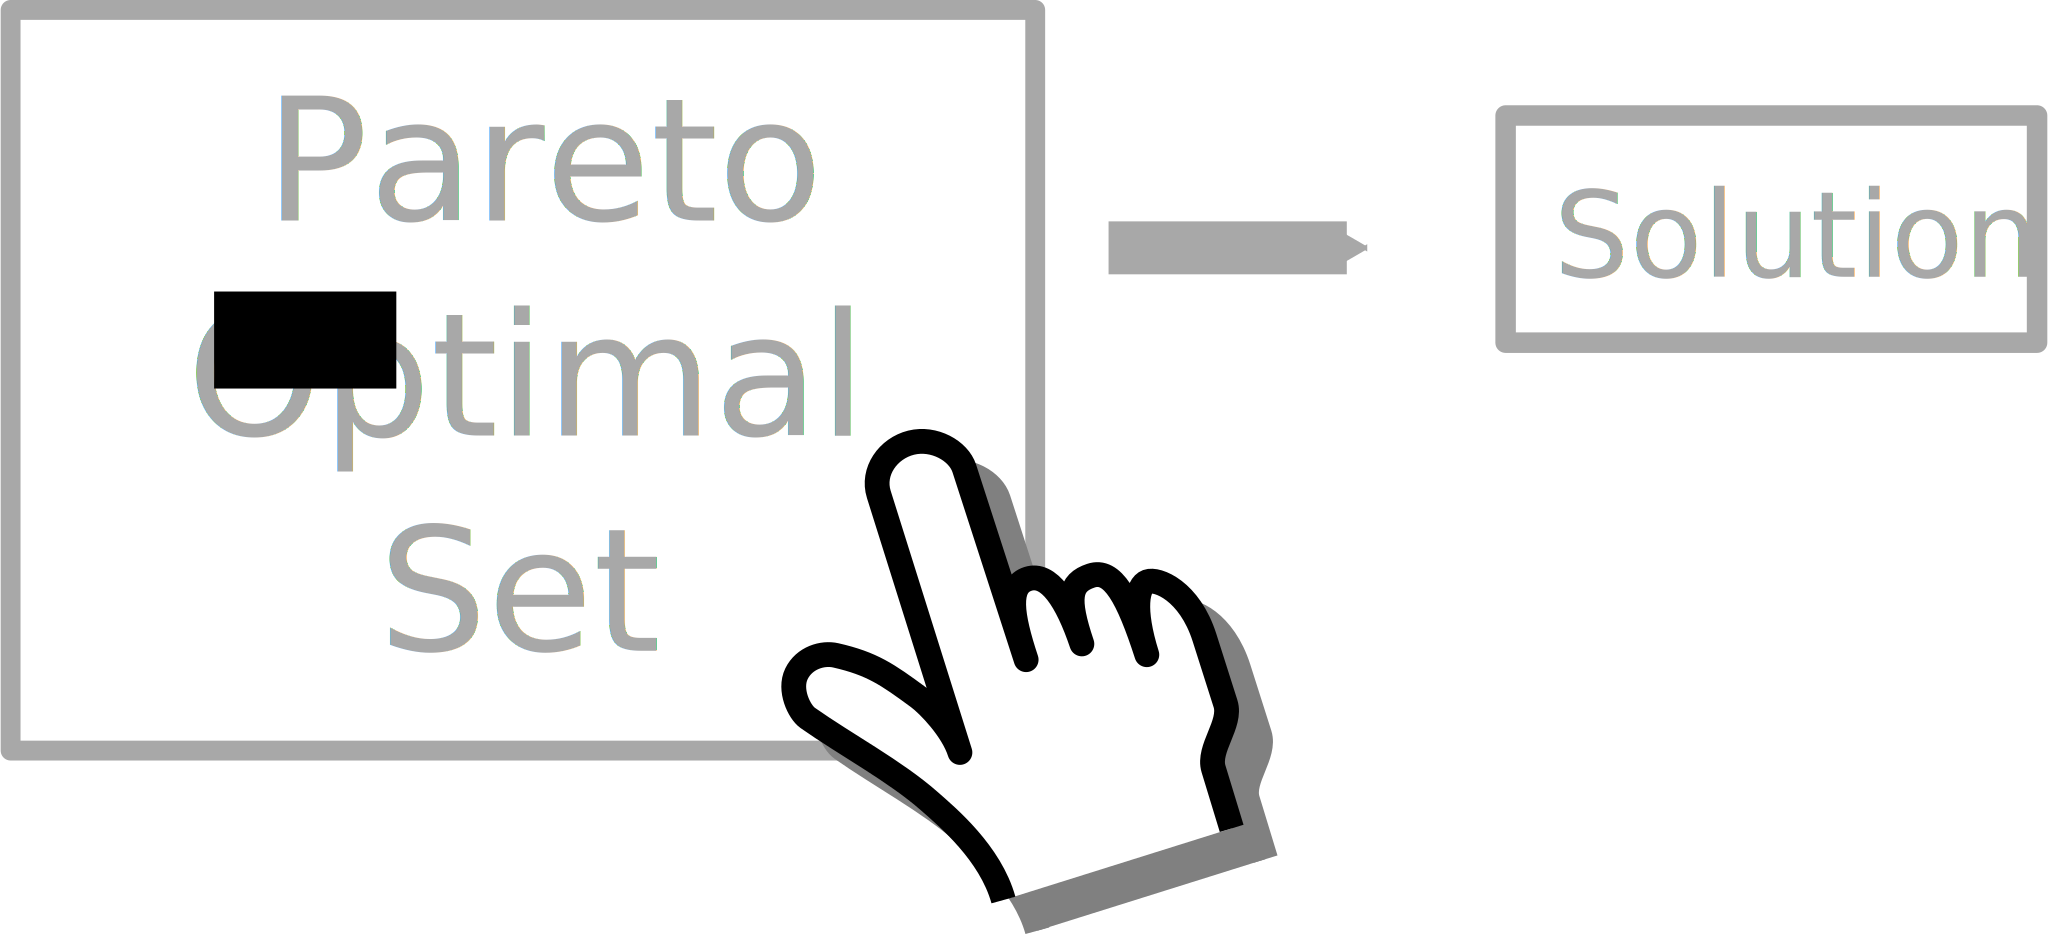
\includegraphics[width=0.6\linewidth]{figure/human_interactive_moo}
%\caption{}
\label{fig:human_interactive_moo}
\end{figure}
\end{frame}

\begin{frame}{Pareto Optimal}{}
\end{frame}

\section{Related work}

\begin{frame}{Graph based approach}{Related work}
Multi-objective A$ ^{*}$
\end{frame}

\begin{frame}{Point-equivalence based approach}{Related work}
\end{frame}



\section{System}
\label{sec:system}

In this paper we use the formulas from Kennedy's most recent definition of PSO~\cite{4223164}.
It can be easily extended to many versions of PSO.
This version of PSO includes a constricted position update rule, a personal best update and a star topology formed by a global best update.
The constricted position update rule is
\begin{subequations}
\label{eq:pso_alg}
\begin{equation}
\label{eq:up_vel}
\begin{aligned}
v_{ij}(k+1) = &  \chi [ v_{ij}(k) 
 + \phi^{P} u^{P}_{ij}(k) (x^{P}_{ij}(k) - x_{ij}(k))\\
 & + \phi^{G} u^{G}_{ij}(k) ( x^{G}_{ij}(k) - x_{ij}(k)) ],
\end{aligned}
\end{equation}
\begin{equation}
\label{eq:up_pos}
x_{ij}(k+1) = x_{ij}(k) + v_{ij}(k+1).
\end{equation}
\end{subequations}
$ x_{ij}(k) $ represents the position of particle $ i $ in dimension $ j $ at time $ k $.
$ v_{ij}(k) $ similarly represents the velocity of particle $ i $ in dimension $ j $ also at time $ k $.
$ x^{G}_{ij}(k) $ and $ x^{P}_{ij}(k) $ are global (actually topology) and personal best positions observed by the swarm and the particle respectively. 
$ u^{G}_{ij}(k) $ and $ u^{P}_{ij}(k) $ are independent random values drawn from $ [0,1] $.
$ \chi \in ( 0, 1 ) $, $ \phi^{P} $ and $ \phi^{G} $ are algorithm parameters.
The personal best update is
\begin{equation}
\label{eq:pb_up}
x_{i}^{P}(k) = \arg \max_{ x \in \{ x_{i}(k), x_{i}^{P}(k-1) \} } f(x).
\end{equation}
The global best update is
\begin{equation}
\label{eq:gb_up}
x_{i}^{G}(k) = \arg \max_{ x \in \{ x_{i}(k), x_{i}^{G}(k-1) \} } f(x).
\end{equation}
The share of the global best leads to a star topology in the swarm.

When particle $ i $ finds a position that is better than the current global best, it updates the global best and its personal best.
The swarm moves to a new global-best stagnation.
In this case, there is $ x_{i}(k) = x_{i}^{P}(k) = x_{i}^{G}(k) $ in the particle.
Equation \eqref{eq:up_vel} becomes
\begin{equation}
v_{ij}(k+1) = \chi [ v_{ij}(k) 
 +( \phi^{P} u^{P}_{ij}(k) + \phi^{G} u^{G}_{ij}(k) ) (x^{G}_{ij}(k) - x_{ij}(k))  ].
\end{equation}
As the inertia of the previous velocity $ v_{ij}(k) $ will decay to zero,
the particle is attracted to $ x^{G}_{ij}(k) $ as $ \phi^{P} u^{P}_{ij}(k) + \phi^{G} u^{G}_{ij}(k) \geq 0 $.
This particle can be viewed as a leader of this swarm.
The topology is given in Figure \ref{fig:leader_follower}.
\begin{figure}[tbph]
\centering
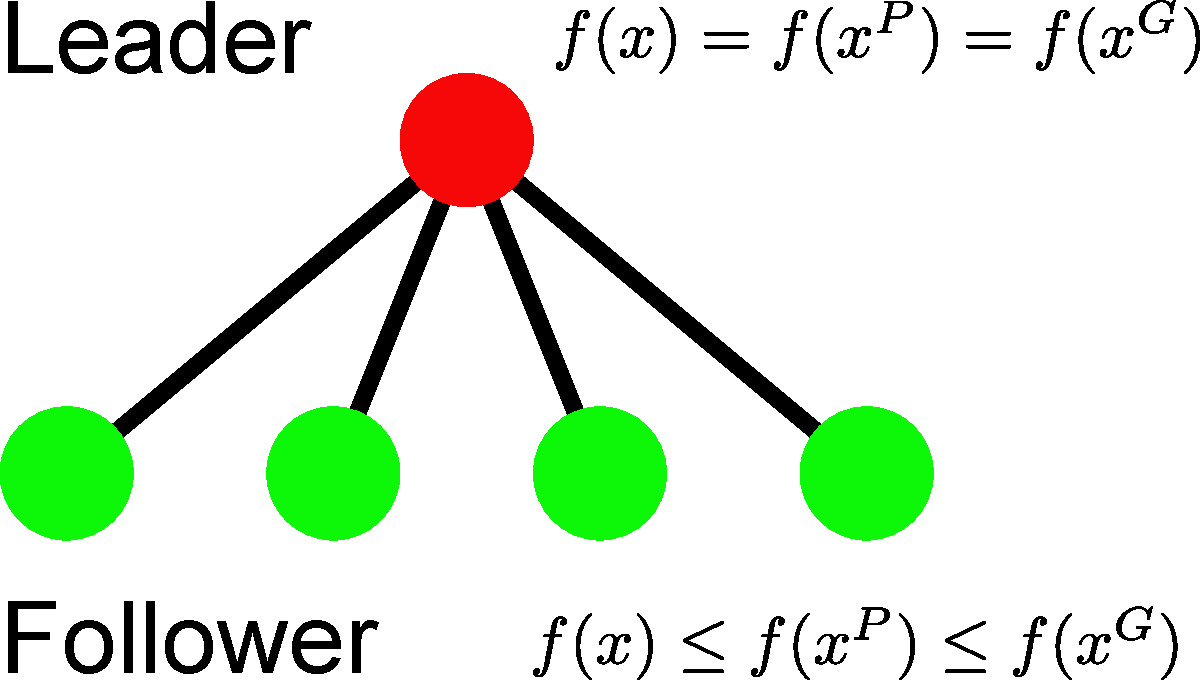
\includegraphics[width=0.5\linewidth]{./fig/leader_follower}
\caption{A leader-follower relationship.}
\label{fig:leader_follower}
\end{figure}

The star topology supports the leader competition among the particles.
The particle that finds a new global best becomes the leader of the swarm.
The other particles are the followers, which are attracted to the leader by the impact of the global best.
By Property \ref{prop:unconverge_neq_gb}, we know that a particle will never stop moving if the personal best and the global best are inconsistent.
Thus, we can view the movements of the followers are sampling in the solution space to solve the inconsistency between its own personal best and the global best.
The input to each particle from the topology of the swarm is only the global best.

\subsection{A feedback cascade model in a particle}

With the global best as the input, we model the behavior of a particle as a \emph{feedback cascade system}.
As shown in Figure \ref{fig:sys_flow}, this system is comprised of two components that form a feedback system structure.
These two components are 
the \emph{input-update component} for the personal best ($ x^{P}_{i}(k) $) and the global best ($ x^{G}_{i}(k) $), 
and the \emph{position-update component} for particle position ($ x_{i}(k+1) $), which depends on the inputs $ x^{G}_{i}(k) $ and $ x^{P}_{i}(k) $ as well as the last position $ x_{i}(k) $.

\begin{figure}
\centering
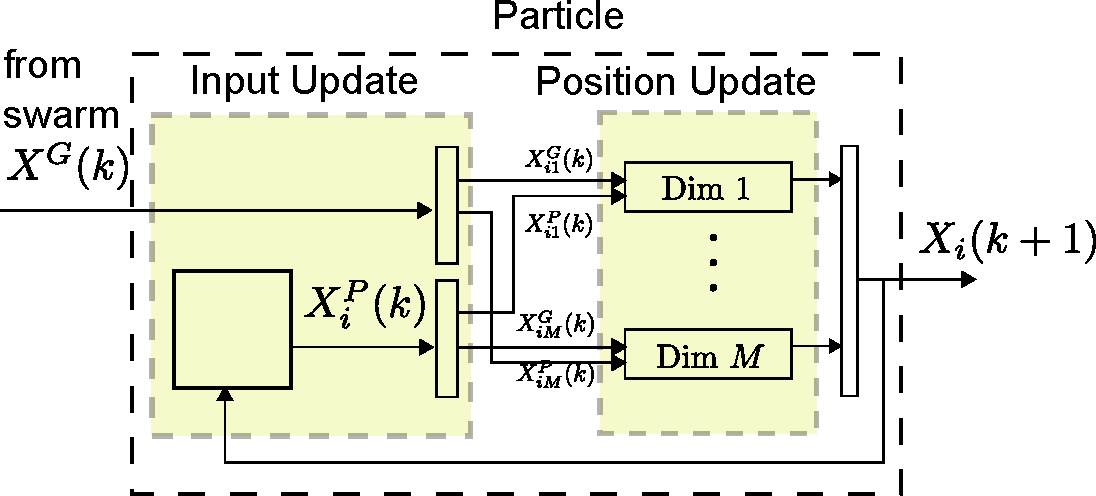
\includegraphics[width=0.85\linewidth]{./fig/sys_flow.pdf}
\caption{System structure of Particle.}
\label{fig:sys_flow}
\end{figure}

\begin{figure}
\centering
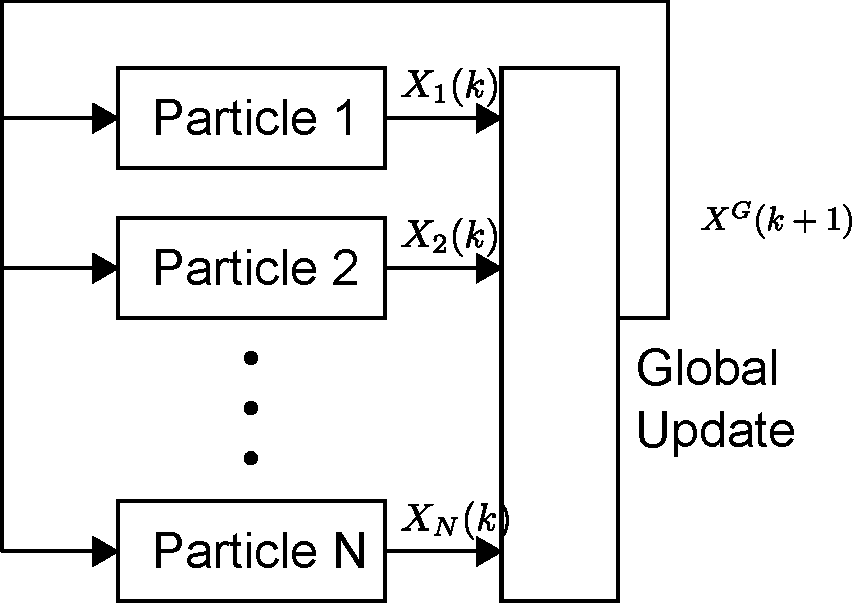
\includegraphics[width=0.6\linewidth]{./fig/pso_sys_flow.pdf}
\caption{System structure of Swarm}
\label{fig:pso_sys_flow}
\end{figure}

In the position-update component, the position at each dimension is updated by using the values from the $ x^{G}_{i}(k) $ and the $ x^{P}_{i}(k) $ in the corresponding dimension.
By Equation \eqref{eq:pso_alg}, we can decompose the position-update component into subcomponent in each dimension.
As shown in Figure \ref{fig:sys_flow}, the subcomponents in the position-update component form a parallel connection.
From \eqref{eq:pso_alg}, we can write a linear form of the position update component in one dimension.
\begin{equation}
\label{eq:pso_up_linalg_simp}
X(k+1) = A(k) X(k) + B(k) U(k)
\end{equation}
with
$ A(k) = \begin{bmatrix}
\chi & - \chi \phi^{G} u^{G}(k) - \chi \phi^{P} u^{P}(k)
\\ 
\chi & 1 - \chi \phi^{G} u^{G}(k) - \chi \phi^{P} u^{P}(k)
\end{bmatrix} $
and
$ B(k) = \begin{bmatrix}
\chi \phi^{G} u^{G}(k) & \chi \phi^{P} u^{P}(k)
\\ 
\chi \phi^{G} u^{G}(k) & \chi \phi^{P} u^{P}(k)
\end{bmatrix} $.
The system state is $ X(k) = [ v(k), x(k) - x^{*} ]^{T} $, and the system input is $ U(k) = [ x^{G}(k) - x^{*} , x^{P}(k) - x^{*} ]^{T} $.
\footnote{$ x^{*} $ means a reference point to the system.
When applying to the PSO, it can be a local optimum, a global optimum, or an estimated optimum.
We use it as a reference point to check the bounds.}
With a new $ x(k+1) $, the personal best update component will update the personal best $ x^{P}(k+1) $ that are fed into the position update component.

The input-update component consists of a \emph{global-best input} and a \emph{personal-best update}.
The personal best and global best are fed into the position-update component as input.
As in Figure \ref{fig:sys_flow}, the global-best input only takes the input from the swarm.
Thus the state to the reference point $ x^{R} $ is $  x^{G}(k) - x^{*} $.
The personal-best update compares the current $ x(k) $ with the $ x^{P}(k-1) $.
If  $ x_{i}(k) $ is better, the personal best is updated with it.
We can write the personal-best update as 
\begin{equation}
\label{eq:pso_input_up}
U = g^{PU}(V)
\end{equation}
with $ U = x^{P}(k) - x^{*} $ 
and $ V = x(k) - x^{R} $
from \eqref{eq:pb_up}. 

In Figure \ref{fig:sys_flow}, the position of a particle is modeled into a system with the input $ x^{G}(k) $ and the output $ x(k) $.
By using this model, we can have the system structure of a swarm in Figure \ref{fig:pso_sys_flow}.
There is a \emph{global update} that reads the states of all the particles and determine whether the global best should be updated.
The global best is fed back to all the particles for the next optimization iteration.



\section{Input-to-State Stability of the Position Update}
\label{sec:iss}

In this section, we briefly review the definition of input-to-state stability (ISS) including both the conditions that guarantee it and the bound that ISS implies\cite{Jiang2001857}. 
We then show that PSO satisfies this definition when the parameters of PSO are set in the requisite range. We also derive the bounds implied by the ISS property.
We use the ISS property in Section \ref{sec:opt_strgy} to find bounds on particle motion.

We first introduce several types of functions \cite{Jiang2001857}.
\begin{itemize}
\item $ K $-function $ \mathbb{K} $ : a function $ \alpha  : [ 0, a ) \rightarrow [ 0, \infty ) $ is continuous, strictly increasing and $ \alpha (0) = 0 $; it is a $ K_{\infty} $-function, if $ \alpha (s) \rightarrow \infty $ as $ s \rightarrow \infty $;
\item $ KL $-function $ \mathbb{KL} $ : a function $ \beta : [ 0, a ) \times [ 0 , \infty ) \rightarrow [ 0, \infty ) $ satisfies:
\begin{enumerate}
\item $ \forall t \geq 0 $, $ \beta (\cdot , t ) $ is a $ K $-function;
\item $ \forall s \geq 0 $, $ \beta (s, \cdot) $ is decreasing and $ \beta(s,t) \rightarrow 0 $ as $ t \rightarrow \infty $.
\end{enumerate}
%\item Positive-definite function: a function $ \gamma (s) > 0, \forall s > 0 $ and $ \gamma (0) = 0 $.
\item ISS-Lyapunov function $ V : \mathbb{R}^{n} \rightarrow \mathbb{R}_{\geq 0} $ satisfies:
\begin{enumerate}
\item $ \exists \alpha_{1}, \alpha_{2} \in \mathbb{K} $ such that 
$ \forall \xi \in \mathbb{R}^{n}, \alpha_{1} ( | \xi | ) \leq V( \xi ) \leq \alpha_{2}  ( | \xi | ) $.
\item $ \exists \alpha_{3} \in \mathbb{K}_{\infty} , \sigma \in \mathbb{K} $ such that $ \forall \xi \in \mathbb{R}^{n}, \forall \mu \in \mathbb{R}^{m}, V( f( \xi, \mu ) ) - V( \xi ) \leq - \alpha_{3} ( | \xi | ) + \sigma ( | \mu | ) $. 
\end{enumerate}
\end{itemize}

\begin{mydef}[Input-to-state stable]\cite{Jiang2001857}
\label{def:iss}
For a discrete-time system
\begin{equation}
\label{eq:dis_nonlinear}
x(k+1) = f( x(k) , u(k) ),
\end{equation}
with $ f(0,0) = 0 $
\footnote{This means that $ x = 0 $ is an equilibrium of the 0-input system.}, the system is \emph{(globally) input-to-state stable} if there exist a $ KL $-function $ \beta  $ and a $ K $-function $ \gamma $ such that, for each input $ u \in l^{m}_{\infty} $ and each $ \xi \in \mathbb{R}^{n} $, it holds that $  \forall k \in \mathbb{Z}^{+} $,
\begin{equation}
\label{eq:def_iss}
| x(k, \xi, u) | \leq \beta (| \xi |, k) + \gamma (|| u ||).
\end{equation}
\end{mydef}

The $ \beta () $ term in equation \eqref{eq:def_iss} defines an initial bound with a decaying property.
The $ \gamma () $ term in equation \eqref{eq:def_iss} defines a bound determined by the input.
This means that the influence $ \beta () $ term gradually decreases to zero and the position is bounded by a range determined by the bound on the input.
An ISS-Lyapunov function, defined above, can be used to prove the input-to-state stability of a system and analyze the state bound\cite{Jiang2001857}.
We will use the ISS-Lyapunov-function approach in the proof given later in this section.

\subsection{Conditions for input-to-state stability for position update in PSO}

Using the definition of the PSO position update as given in equation \eqref{eq:pso_up_linalg_simp}, PSO can be shown to be ISS as defined in definition \ref{def:iss}.

\begin{mythm}
\label{thm:iss}
The system \eqref{eq:pso_up_linalg_simp} is input-to-state stable, when $ | \lambda_{\max} ( A(k) ) | < 1 $.
%The system \eqref{eq:pso_up_linalg_simp} is input-to-state stable, if there exists a symmetric positive definite matrix $ P $ and a symmetric positive definite matrix $ Q' $ that has $ A(k)^{T} P A(k) - P = - Q(k) \leq - Q' $.
\begin{proof}

Let $ P $ be an identity matrix.
As $ | \lambda_{\max} ( A(k) ) | < 1 $, we have
$ \lVert A^{T}(k) P A(k) \rVert \leq \lVert P \rVert \lVert A(k) \rVert^{2} \leq \lVert P \rVert | \lambda_{\max} ( A(k) ) |^{2} < \lVert P \rVert $.
Because $ P $ is an identity matrix it is positive definite, and thus $ A^{T}(k) P A(k) $ is positive definite or positive semi-definite by definition.
So by positive definite ordering we have $ A^{T}(k) P A(k) < P $.

Let $ -Q(k) = A^{T}(k) P A(k) - P $. Since $ A^{T}(k) P A(k) < P $ then $ - Q(k) < 0 $ furthermore $ \exists Q' \forall k, Q(k) > Q' > 0 $. 

By the Lemma 3.5 in \cite{Jiang2001857}, if we can show that a proposed positive definite Lyapunov function is an ISS-Lyapunov function, then the system is ISS.

Define a Lyapunov function
\begin{equation}
\label{eq:lyapunov_v}
V( X(k) ) = X^{T} (k) P X(k).
\end{equation}
We can have
$
\lambda_{min}(P) | X(k) |^{2} \leq V( X(k) )\leq \lambda_{max}(P) | X(k) |^{2}
$ and $ \lambda_{min}(P) = \lambda_{max}(P) $.

Let $ \alpha_{1} ( \xi )= \lambda_{min} \xi^{2} $
and 
$ \alpha_{2} ( \xi )= \lambda_{max} \xi^{2} $,
we have $ V(x) $ satisfying condition 1 of the ISS-Lyapunov function definition.

By applying equation \eqref{eq:pso_up_linalg_simp} to $ V( X(k+1) ) - V( X(k) ) $, we have
\begin{equation}
\label{eq:lyapunov_delta2}
\begin{aligned}
& V( X(k+1) ) - V( X(k) ) \\
= & - X^{T}(k) [ A^{T}(k) P A(k) - P ] X(k) \\
& + 2 X^{T}(k)  A^{T}(k) P B(k) U(k) + U^{T}(k) B^{T}(k) P B(k) U(k) \\
\leq & - X^{T}(k) Q' X(k) + 2 X^{T}(k)  A^{T}(k) P B(k) U(k) \\
& + U^{T}(k) B^{T}(k) P B(k) U(k) \\
\leq & - \lambda_{min}(Q') | X(k) |^{2} + 2  \lVert A^{T}(k) P B(k) \rVert | U(k) | | X(k) | \\
& + \lVert B^{T}(k) P B(k) \rVert | U(k) |^{2}.
\end{aligned}
\end{equation}

By completing the square, we have
\begin{equation}
\label{eq:lyapunov_delta4}
\begin{aligned}
& V( X(k+1) ) - V( X(k) ) \\
\leq & - \frac{1}{2} \lambda_{min}(Q') | X(k) |^{2} \\
& + \left[ \frac{2 \lVert A^{T}(k) P B(k) \rVert^{2}}{ ( \lambda_{min}(Q') )^{2} } + \lVert B^{T}(k) P B(k) \rVert \right] | U(k) |^{2}. 
\end{aligned}
\end{equation}

Because $ u^{P}(k) \in [0, 1] $, there exist an $ A' $ and $ B' $ such that $ \lVert A(k) \rVert \leq \lVert A' \rVert $ and $ \lVert B(k) \rVert \leq \lVert B' \rVert $.
We have $ \lVert A^{T}(k) P B(k) \rVert \leq \lVert A' \rVert \lVert P \rVert \lVert B' \rVert $ and $ \lVert B^{T}(k) P B(k) \rVert \leq \lVert P \rVert \lVert B' \rVert^{2} $.

Since the identity matrix $ P $ has $ || P || = 1 $:
\begin{equation}
\label{eq:lyapunov_delta5}
\begin{aligned}
& V( X(k+1) ) - V( X(k) ) \\
\leq & - \frac{1}{2} \lambda_{min}(Q') | X(k) |^{2} + [ \frac{2 \lVert A' \rVert^{2} \lVert B' \rVert^{2}}{ ( \lambda_{min}(Q') )^{2} } + \lVert B' \rVert^{2} ] | U(k) |^{2}.
\end{aligned}
\end{equation}

Let
$ \alpha_{3} ( \xi )= \frac{1}{2} \lambda_{min}(Q') \xi^{2} $,
and
$ \sigma ( \xi ) = [ \frac{2 \lVert A' \rVert^{2} \lVert B' \rVert^{2}}{ ( \lambda_{min}(Q') )^{2} } +  \lVert B' \rVert^{2} ] \xi^{2} $.
Thus we have $  V( X(k+1) ) - V( X(k) ) $ satisfying condition 2 of the ISS-Lyapunov function definition and
so \eqref{eq:lyapunov_v} is an ISS-Lyapunov function.
Using Lemma 3.5 in \cite{Jiang2001857}, the position update component of PSO (equation \eqref{eq:pso_up_linalg_simp}) is input-to-state stable.

\end{proof}
\end{mythm}

Note that in using equation \eqref{eq:pso_up_linalg_simp},
$ [ v(k), x(k) - x^{*} ]^{T} = [0, 0]^{T} $ is an equilibrium position when the input $ [ x^{G}(k) - x^{*} , x^{P}(k) - x^{*} ]^{T} = [0, 0]^{T} $.
For an arbitrary optimization problem $ x^{*} $ would typically not be at the origin. 
In such a problem, input-to-state stability means that the boundaries of $ | v(k) | $ and $ | x(k) - x^{*} | $ would be transformed and thus determined by $ | x^{G}(k) - x^{*} | $ and $ | x^{P}(k) - x^{*} | $,
but the properties of ISS still apply independent of where the function is centered.

Having proven that PSO is ISS we can now state a bound on particle position.

\begin{mycoro}
\label{coro:state_bound}
Given the bound on the input $ || u || $ in the position update component, we have the bound on the particle position from equation \eqref{eq:pso_up_linalg_simp}.
\begin{equation}
\label{eq:state_bound}
\forall k, 
| x(k) - x^{*} | \leq \max ( | x(0) - x^{*} | , \gamma ( | [ x^{G}(k) - x^{*}, x^{P}(k) - x^{*} ]^{T} | ) ),
\end{equation}
in which $ \gamma = \alpha_{3}^{-1} \circ \sigma $.

The $ \max $ part is needed to account for the effect of the starting point, represented by the first parameter. Eventually the effect of the starting point no longer affects the system, formally:
\begin{equation}
\label{eq:state_bound:conv}
\exists T, \forall k \geq T, 
|  x(k) - x^{*} | \leq \gamma ( | [ x^{G}(k) - x^{*}, x^{P}(k) - x^{*} ]^{T} | ).
\end{equation}
\begin{proof}
This is obtained from Remark 3.7 in \cite{Jiang2001857} and by choosing $ P $ be a symmetric identity matrix.
Furthermore we drop the velocity part becuase $ | x(k) - x^{*} | \leq | [ v(k), x(k) - x^{*} ]^{T} | $.
\end{proof}
\end{mycoro}

Figure \ref{fig:boundary} gives an example on how a particle's boundary is determined by the personal best and global best.

\begin{figure}
\centering
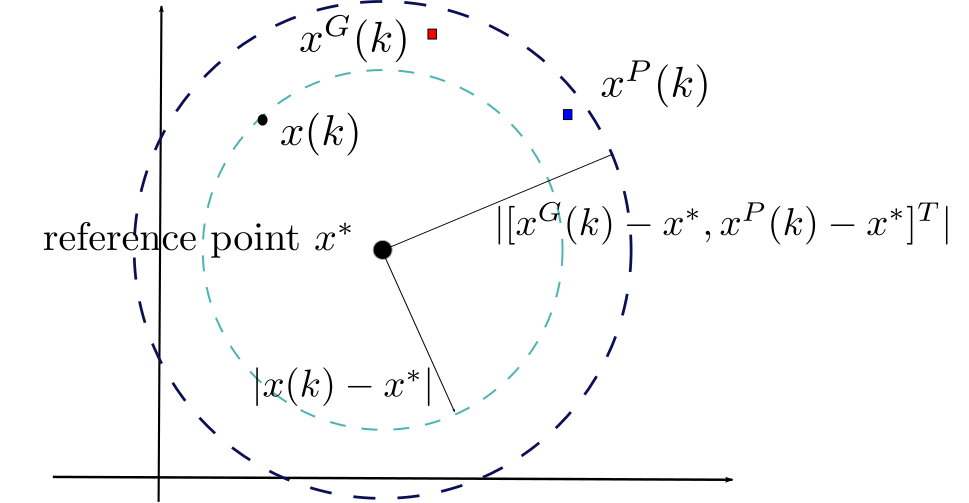
\includegraphics[width=0.9\linewidth]{./figure/boundary}
\caption{A bound on a particle's position by a reference point $ x^{*} $ from Equation \ref{eq:state_bound:conv}.
The ratio of wo radii indicates $ \gamma $.}
\label{fig:boundary}
\end{figure}

\begin{mycoro}
\label{coro:param_unit_disc}
Write $ A(k) = 
\begin{bmatrix}
\chi & - \chi \phi \\
\chi & 1 - \chi \phi
\end{bmatrix}
$, in which
$ \phi \in [0,  \phi^{P} + \phi^{G} ] $ and $ \chi \in ( 0, 1 ) $.
When $ \phi \in (0 , \frac{2(1+\chi)}{\chi} ) $, the system \eqref{eq:pso_up_linalg_simp} is input-to-state stable.
\begin{proof}
Let $ a = (1 + \chi) - \chi \phi $. 
The eigenvalues of $ A(k) $ are
$ \lambda = \frac{ a \pm \sqrt{ a^{2} - 4 \chi } }{2} $.

\begin{enumerate}
\item If $ a^{2} \geq 4 \chi $, we have $ a \geq 2 \sqrt{\chi} $ or $ a \leq - 2 \sqrt{\chi} $.

If $ a \geq 2 \sqrt{\chi} $, then $ | \lambda_{\max} | < 1 $ derives $ 0 < \frac{a-\sqrt{a^{2}-4\chi}}{2} \leq \frac{a+\sqrt{a^{2}-4\chi}}{2} < 1 $.
It means that $ 2 \sqrt{ \chi } \leq a < 1 + \chi $.

If $ a \leq 2 \sqrt{\chi} $, then $ | \lambda_{\max} | < 1 $ derives $ -1 < \frac{a-\sqrt{a^{2}-4\chi}}{2} \leq \frac{a+\sqrt{a^{2}-4\chi}}{2} < 0 $.
It means that $ - (\chi+1) < a \leq - 2 \sqrt{\chi} $.

\item If $ a^{2} \geq 4 \chi $, we have $ - 2 \sqrt{\chi} < a < 2 \sqrt{\chi} $.

$ | \lambda_{\max} | < 1 $ derives $ \frac{ a^{2} }{4} + \frac{ a^{2} - 4\chi }{4} < 1 $.
It means that $ - 2 \sqrt{ 2(1+\chi) } < a < 2 \sqrt{ 2(1+\chi) } $.
Because $ \sqrt{ 2(1+\chi) } > 2 \sqrt{ \chi } $, we have $ - 2 \sqrt{\chi} < a < 2 \sqrt{\chi} $.
\end{enumerate}
Combining these two cases, we have  $ - (1 + \chi) < a < 1 + \chi $.
It equals to $ \phi \in (0 , \frac{2(1+\chi)}{\chi} ) $.

\end{proof}
\end{mycoro}

Figure \ref{fig:paramSpace} shows the parameter space.
The x-axis is $ \phi = \phi^{P} + \phi^{G} $ and the y-axis is $ \chi $.
The stable region in red is obtained from eigenvalue test on Theorem \ref{thm:iss} and the yellow boundary is obtained from Corollary \ref{coro:param_unit_disc}.
\begin{figure}
\centering
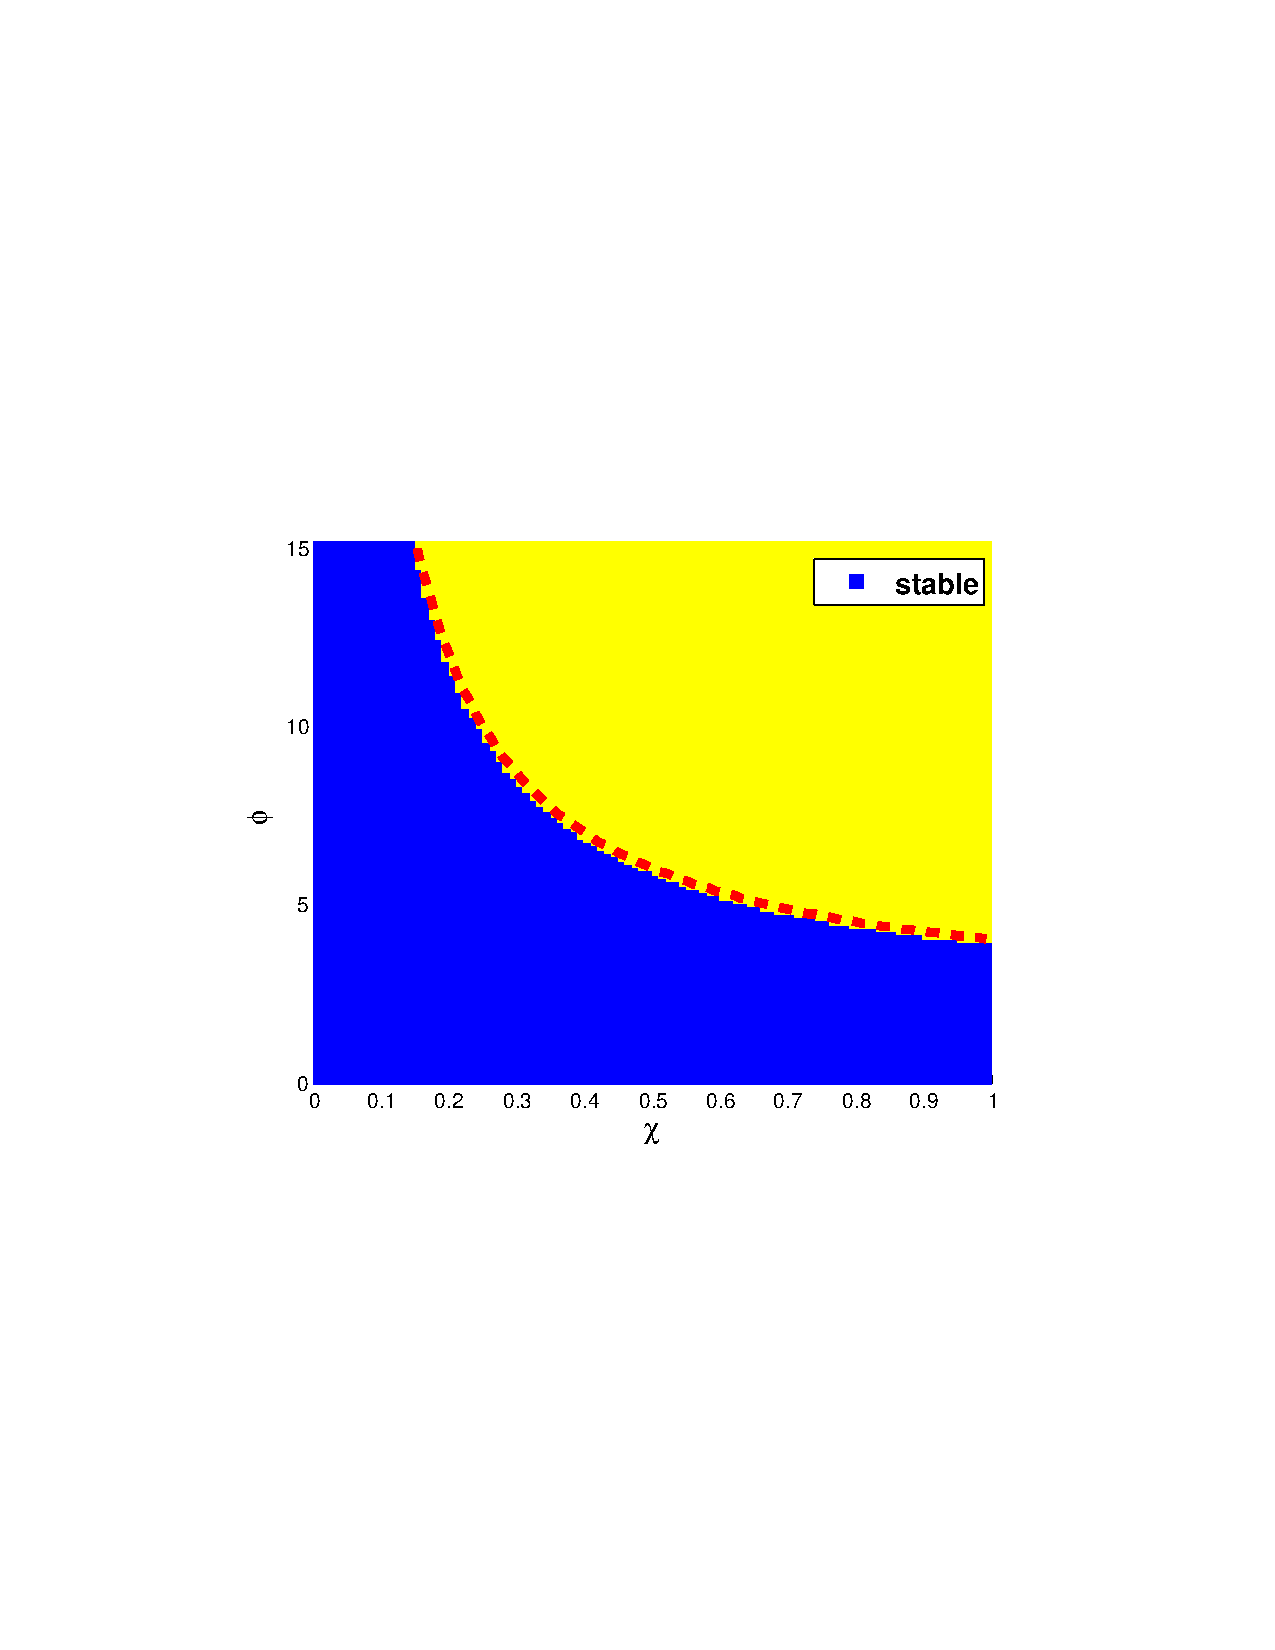
\includegraphics[width=0.9\linewidth]{./figure/param2}
\caption{Parameter space}
\label{fig:paramSpace}
\end{figure}

\begin{figure}
\centering
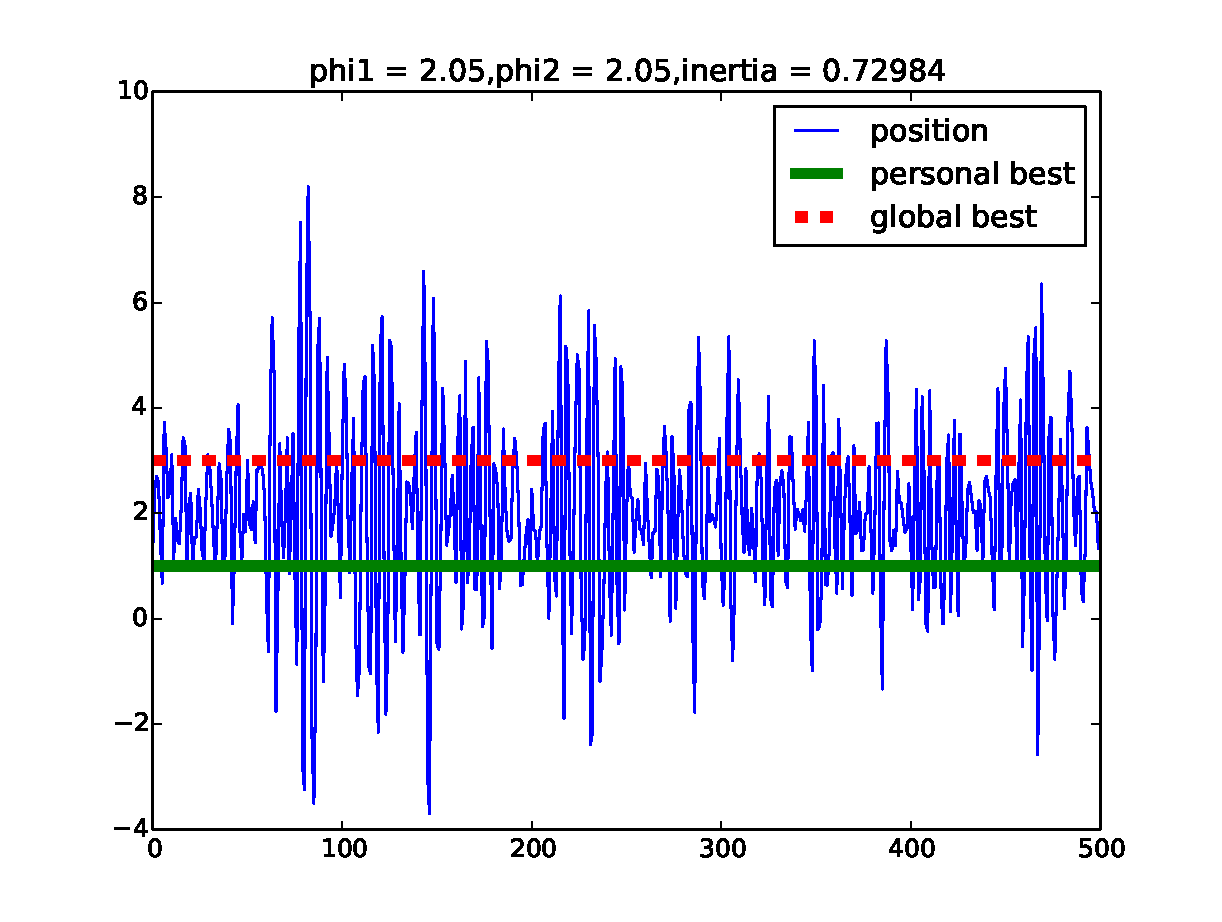
\includegraphics[width=\linewidth]{./figure/bound_case_1}
\caption{Parameters in the margin of stable region.}
\label{fig:bound_case:a}
\end{figure}

\begin{figure}
\centering
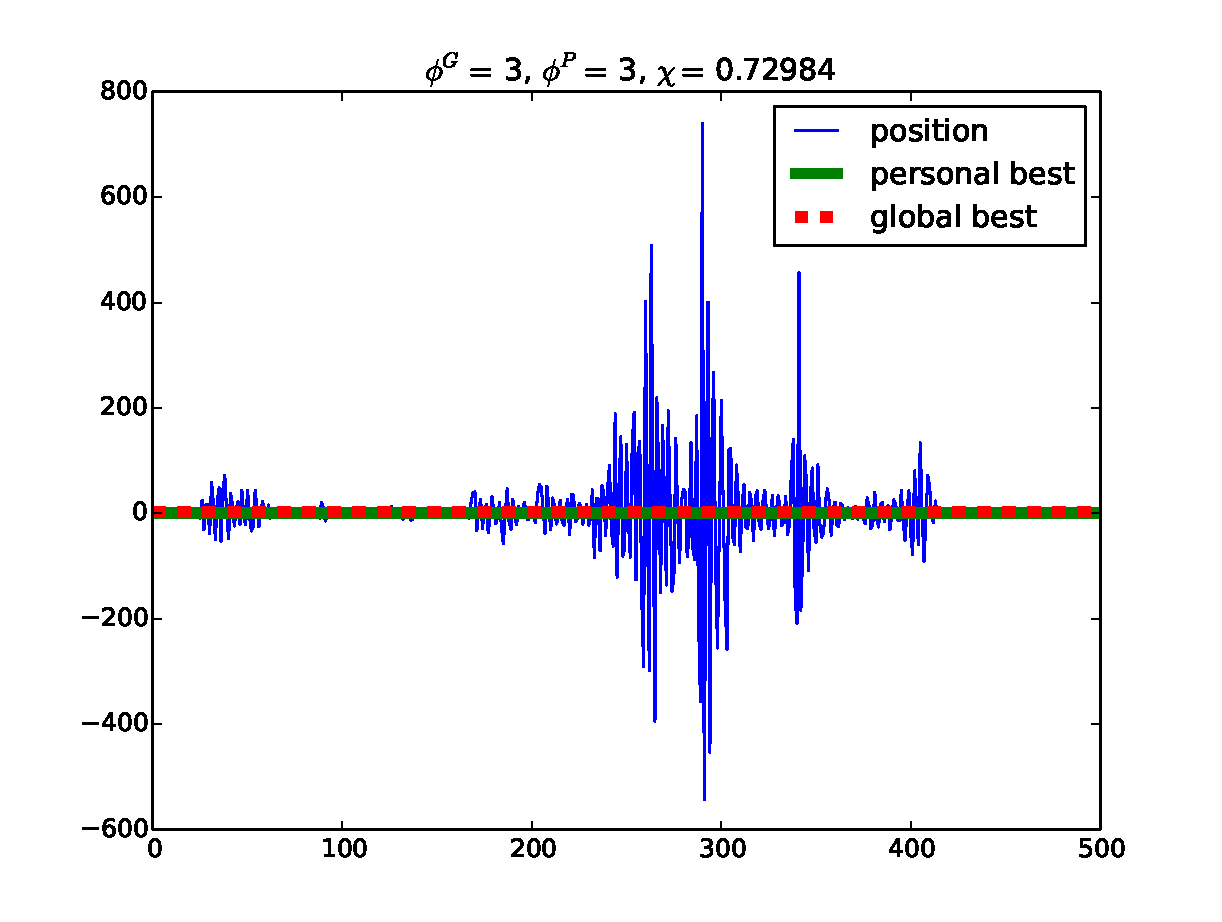
\includegraphics[width=\linewidth]{./figure/bound_case_2}
\caption{Parameters not in the stable region.}
\label{fig:bound_case:b}
\end{figure}

\begin{figure}
\centering
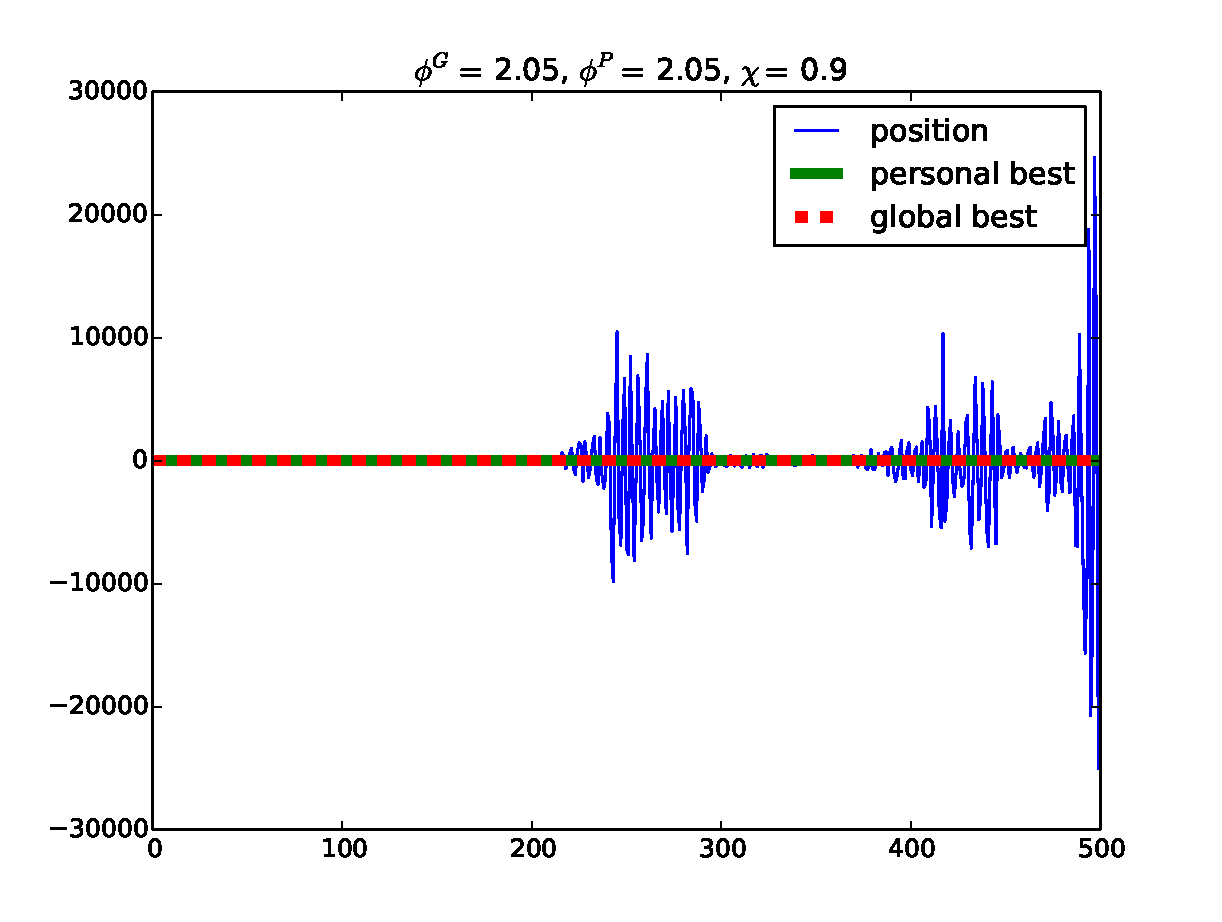
\includegraphics[width=\linewidth]{./figure/bound_case_3}
\caption{Parameters not in the stable region.}
\label{fig:bound_case:c}
\end{figure}

\begin{figure}
\centering
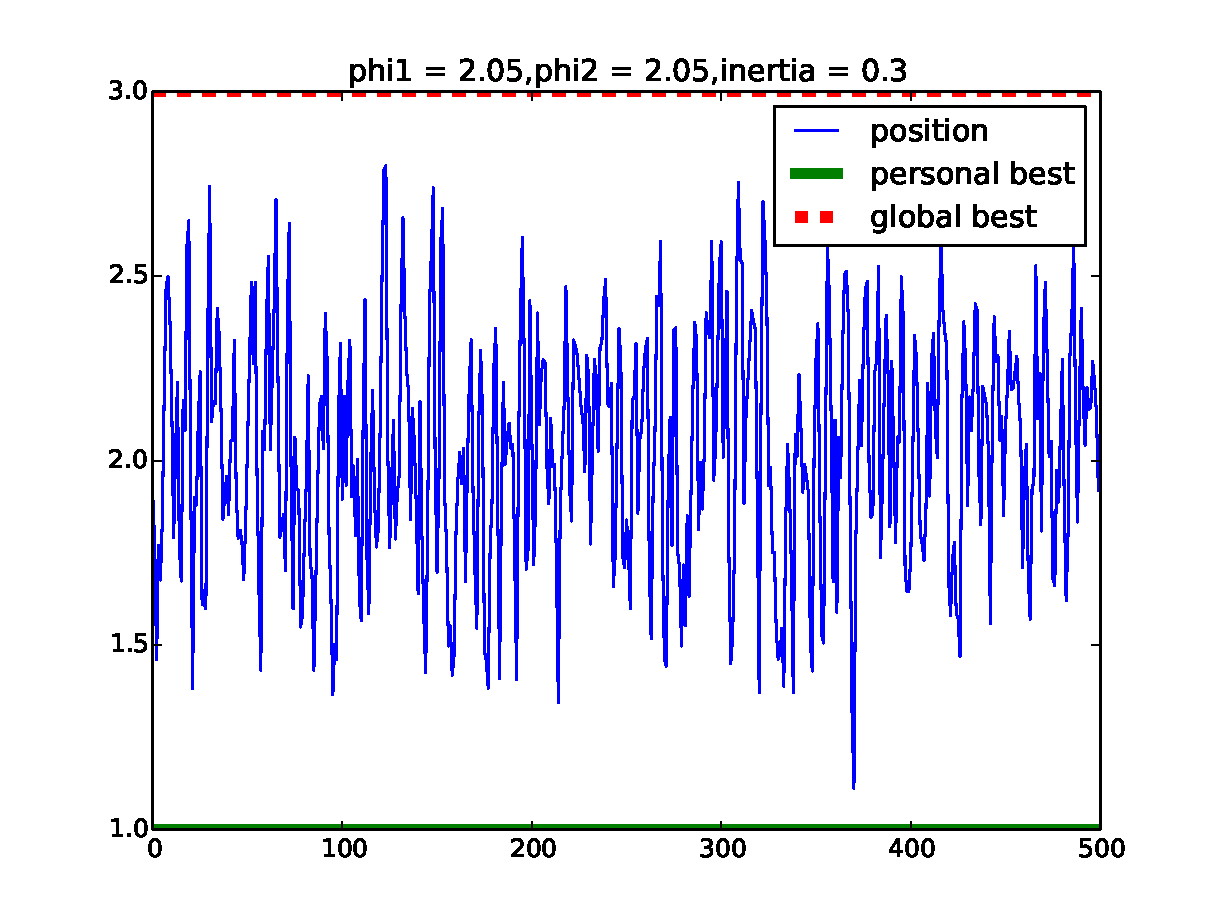
\includegraphics[width=\linewidth]{./figure/bound_case_4}
\caption{Parameters in the stable region.}
\label{fig:bound_case:d}
\end{figure}

\begin{figure}
\centering
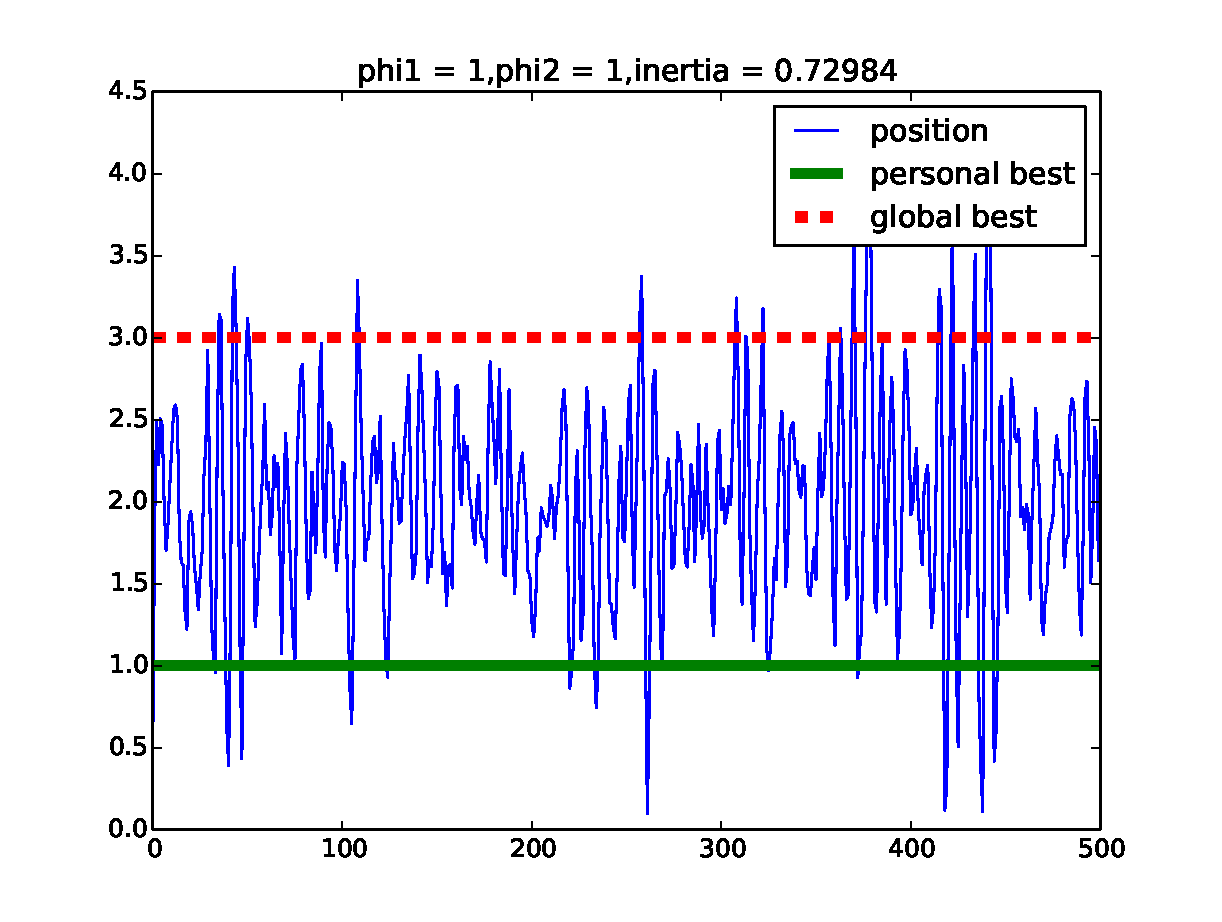
\includegraphics[width=\linewidth]{./figure/bound_case_5}
\caption{Parameters in the stable region.}
\label{fig:bound_case:e}
\end{figure}




\section{Particle analysis}
\label{sec:particle}

In this section, we analyze the behavior of a single particle in a swarm.
In a single stagnation, the global best is unchanged.
Thus we make the global best as the constant.
We are interested with 
\begin{itemize}
\item whether the particle converges to the global best;
\item and the probability that the particle find a new global best.
\end{itemize}

In order to understand how the particle converges to the global best, we let $ x^{G} $ be the reference position and get Equation \eqref{eq:rel_gb}.

\begin{equation}
\label{eq:rel_gb}
\begin{aligned}
\begin{bmatrix}
v(k+1) \\
x(k+1) - x^{G}
\end{bmatrix}
 = A(k) 
\begin{bmatrix}
v(k) \\
x(k) - x^{G}
\end{bmatrix}
+ B(k) 
\begin{bmatrix}
0 \\
x^{P}(k) - x^{G}
\end{bmatrix}
\end{aligned}
\end{equation}

By Theorem \ref{coro:state_bound}, we know that $ \lVert x(k) - x^{G} \rVert $ indicates the distance to the global best, which depends on  $ \lVert x^{P}(k) - x^{G} \rVert $.

\subsection{Unimodal fitness distribution}

A unimodal fitness distribution is most typical.
It provides a partial monotonic form and most of the cases the final convergence happens on a unimodal fitness distribution.
Any other form can usually be viewed as a combination of unimodalities as well.

When the global best is already the optimal solution, there is no chance for the particle to find a better solution and trigger a new global best.
The particle should gradually converge to the global best if the position update component is input-to-state stable, as in Lemma \ref{lem:singleHill:particle:converge}.

\begin{mylem}
\label{lem:singleHill:particle:converge}
In a unimodal case, when $ x^{G} = x^{*} $, the particle will converge to $ x^{G} $ if the update component of the particle is input-to-state stable.
\begin{proof}
When $ x^{G} = x^{*} $, the input update component is also input-to-state stable.
The serial connection of two ISS components still reserves input-to-state stability.
As the input is zero by $ \lVert x^{G} - x^{*} \rVert = 0 $, $ x(k) - x^{*} $ will converge to zero.
\end{proof}
\end{mylem}

When the global best is not yet the optimal solution, the convergence of the particle cannot be guaranteed.
If the particle accidentally reaches into a region that the fitness is better than the current global best, a new global best is found.
The particle might either runs stochastically in a region that the fitness is worse than both the personal best and the global best.
If the particle at least gets into a position that is better than the current personal best, the personal best will be updated. 
We notice that the particle should never stop at the current global best $ x^{G} $, which is stated in Lemma \ref{lem:singleHill:particle:nonstop}.

\begin{mylem}
\label{lem:singleHill:particle:nonstop}
In a unimodal case, if $ x^{G} \not = x^{*} $, a particle will never stop at $ x^{G} $. 
\footnote{The precision cut-off in implementation is ignored.}
\begin{proof}
Consider the velocity $ v(k+1) $ consists of two parts, inertia $ \chi v(k) $ and attractive force $ \chi \phi^{P} (x^{P}(k) - x(k) ) + \chi \phi^{G} ( x^{G} - x(k) ) $.
While the particle moves into $ x^{G} $, the attractive force becomes zero but the inertia still exists, due to the velocity moves the particle into this current position.
\end{proof} 
\end{mylem}

By Lemma \ref{lem:singleHill:particle:nonstop}, we can prove that the particle will finally get to a position that is at least better than the current global best if given enough run time.
We have Theorem \ref{thm:singleHill:particle:better}.

\begin{mythm}
\label{thm:singleHill:particle:better}
In a unimodal case, the particle will almost surly find a $ \hat{x^{*}} $ that $ f(\hat{x^{*}}) > f(x^{G}) $ if $ f( x^{G} ) < f( x^{*}) $.
\begin{proof}
Because the particle cannot stop at $ x(k) = x^{G} = x^{P} $.
It will finally arrives into a region that $ f(x) > f(x^{G}) $.

As in Figure \ref{fig:categorize_regions}, the solution space will be divided into three types of regions by the global best and the personal best.
\begin{itemize}
\item $ f(x) > f(x^G) $
Once a particle gets into this region, it updates both global best and personal best. 
It becomes a leader of the swarm.
\item $ f(x^{G}) > f(x) > f(x^{P}) $
Once a particle gets into this region, it updates only the personal best.
The solution space is then re-divided.
\item $ f(x) < f(x^{P}) $
When a particle is in this region, it only moves as a random walk.
\end{itemize}

\begin{figure}
\centering
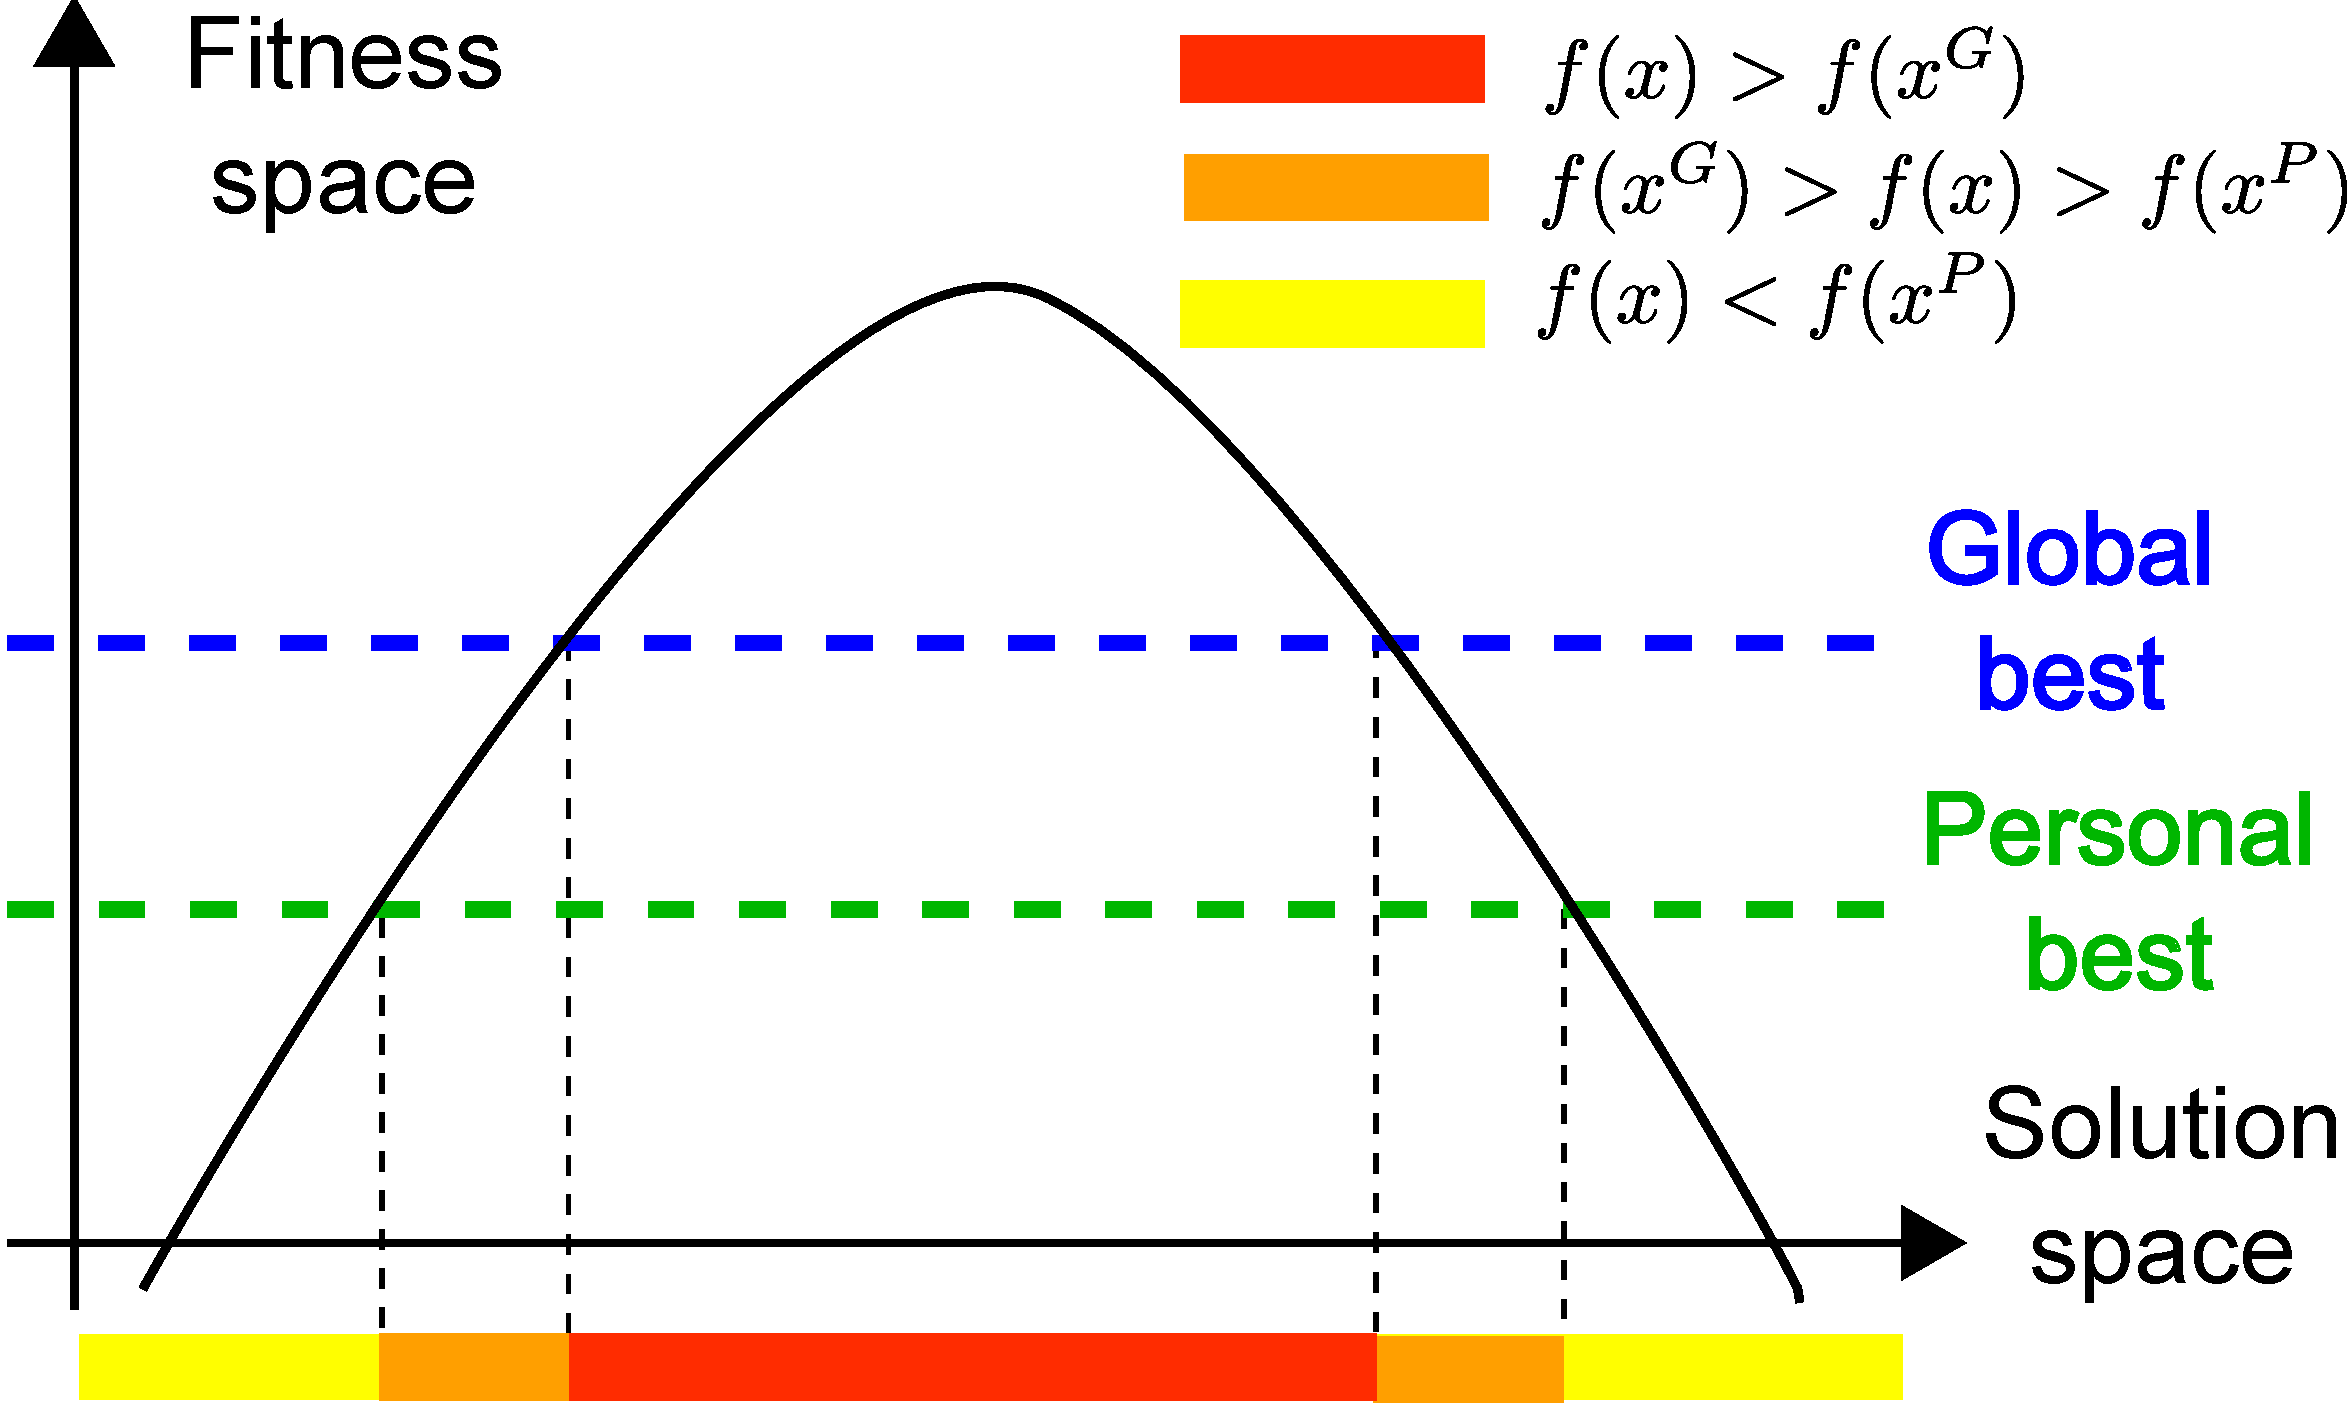
\includegraphics[width=0.7\linewidth]{./fig/categorize_regions}
\caption{How global best and personal best divide the solution space.}
\label{fig:categorize_regions}
\end{figure}

The result of the movement of a particle is determined by which region of the solution space it moves in.
The states of the particle can be defined as
\begin{itemize}
\item \textbf{A} [$ f(x) \leq f(x^{P}) \leq f(x^{G}) $]
\item \textbf{B} [$ f(x) = f(x^{P}) \leq f(x^{G}) $] 
\item \textbf{C} [$ f(x) = f(x^{P}) \leq f(x^{G}) \land v > 0 $]
\item \textbf{D} [$ f(x) = f(x^{P}) \leq f(x^{G}) \land v = 0 $]
\item \textbf{E} [$ f(x) > f(x^{P}) = f(x^{G}) $]
\end{itemize}


\begin{figure}[tbph]
\centering
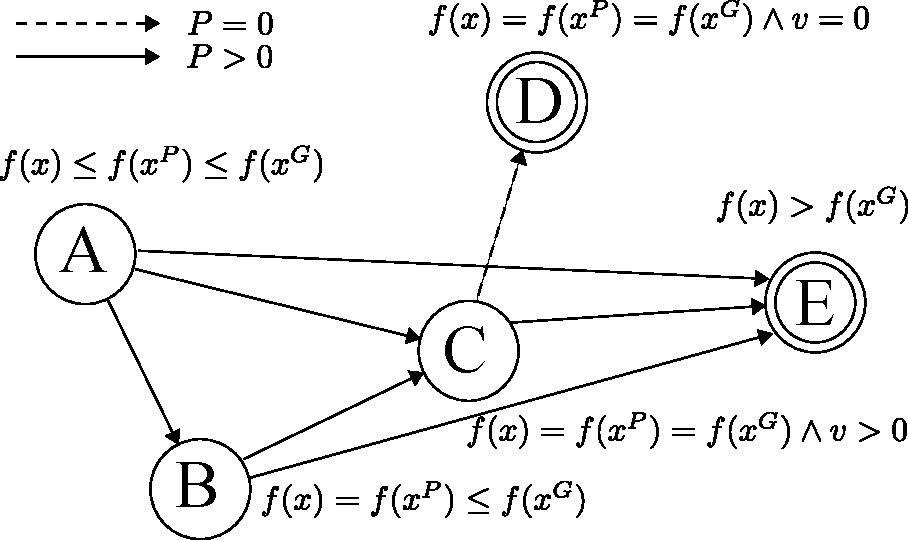
\includegraphics[width=0.7\linewidth]{./fig/fsm}
\caption{}
\label{fig:fsm}
\end{figure}

\end{proof}
\end{mythm}

\subsubsection{Simulation on unimodal case}

\begin{figure}[ht]
\centering
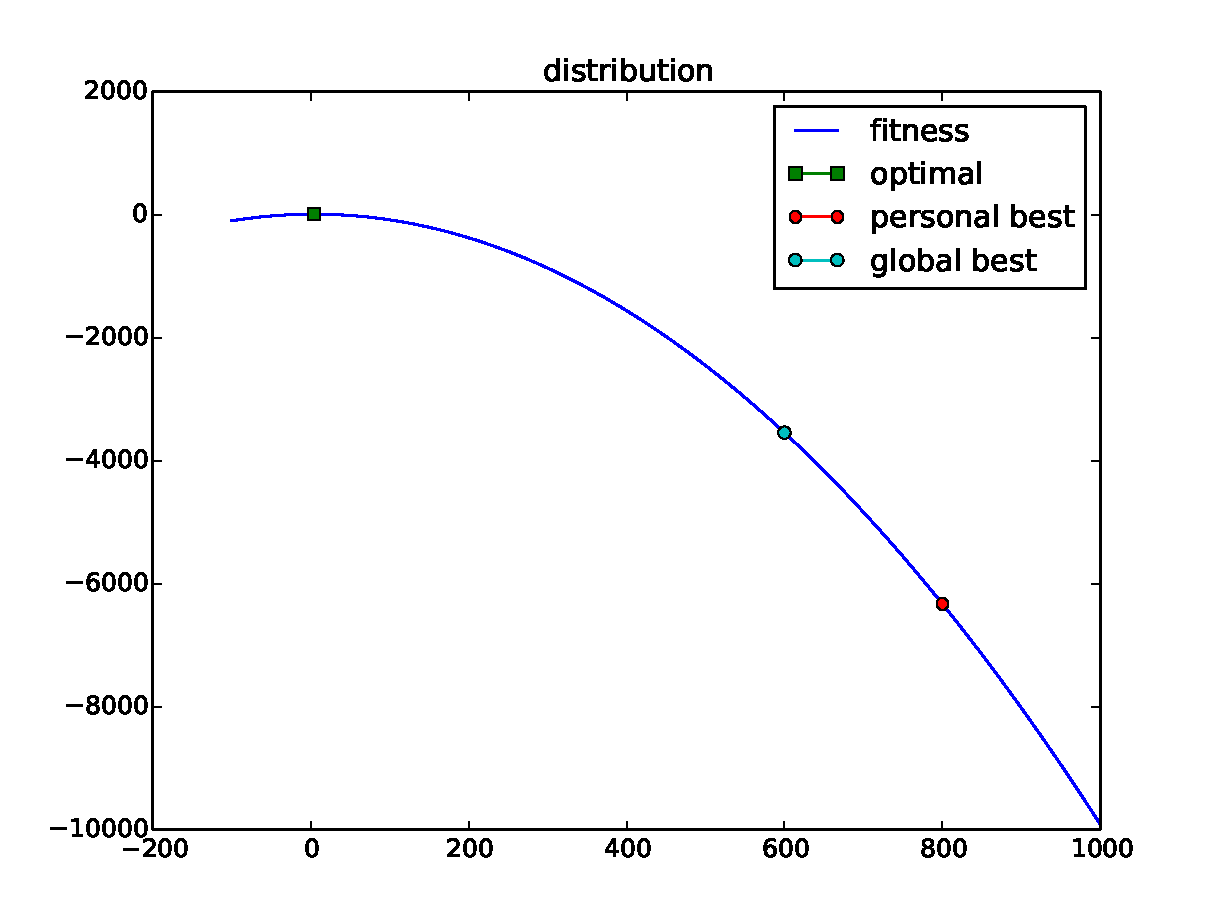
\includegraphics[width=.7\linewidth]{./simfig/case1/distribution1}
\label{fig:case1-1:distribution} 
\end{figure}

\begin{figure}[ht]
\centering
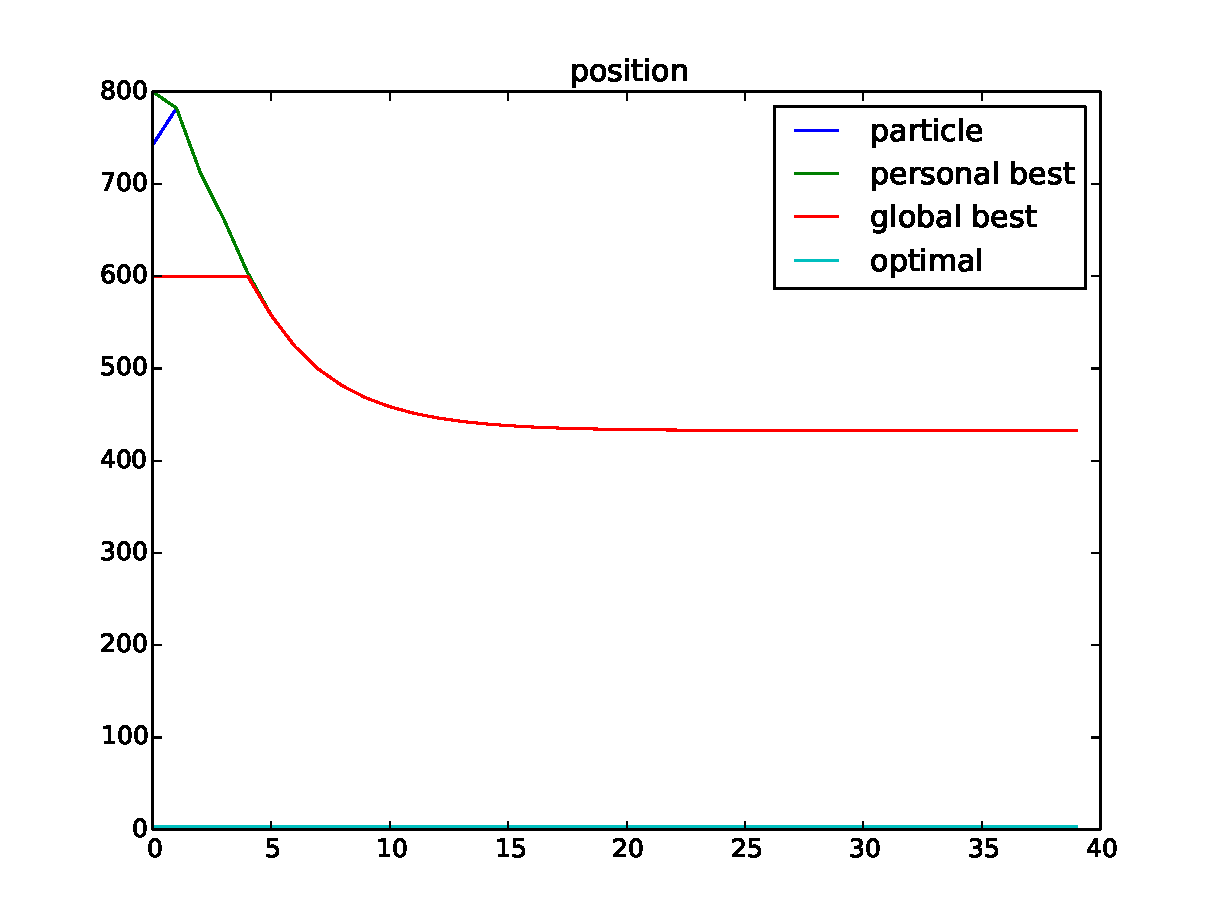
\includegraphics[width=.7\linewidth]{./simfig/case1/position1-1} 
\label{fig:case1-1:position}
\caption{$ \chi = 0.72984 , \phi^{P} = 2.05 , \phi^{G} = 2.05 $ }
\end{figure}

\begin{figure}[ht]
\centering
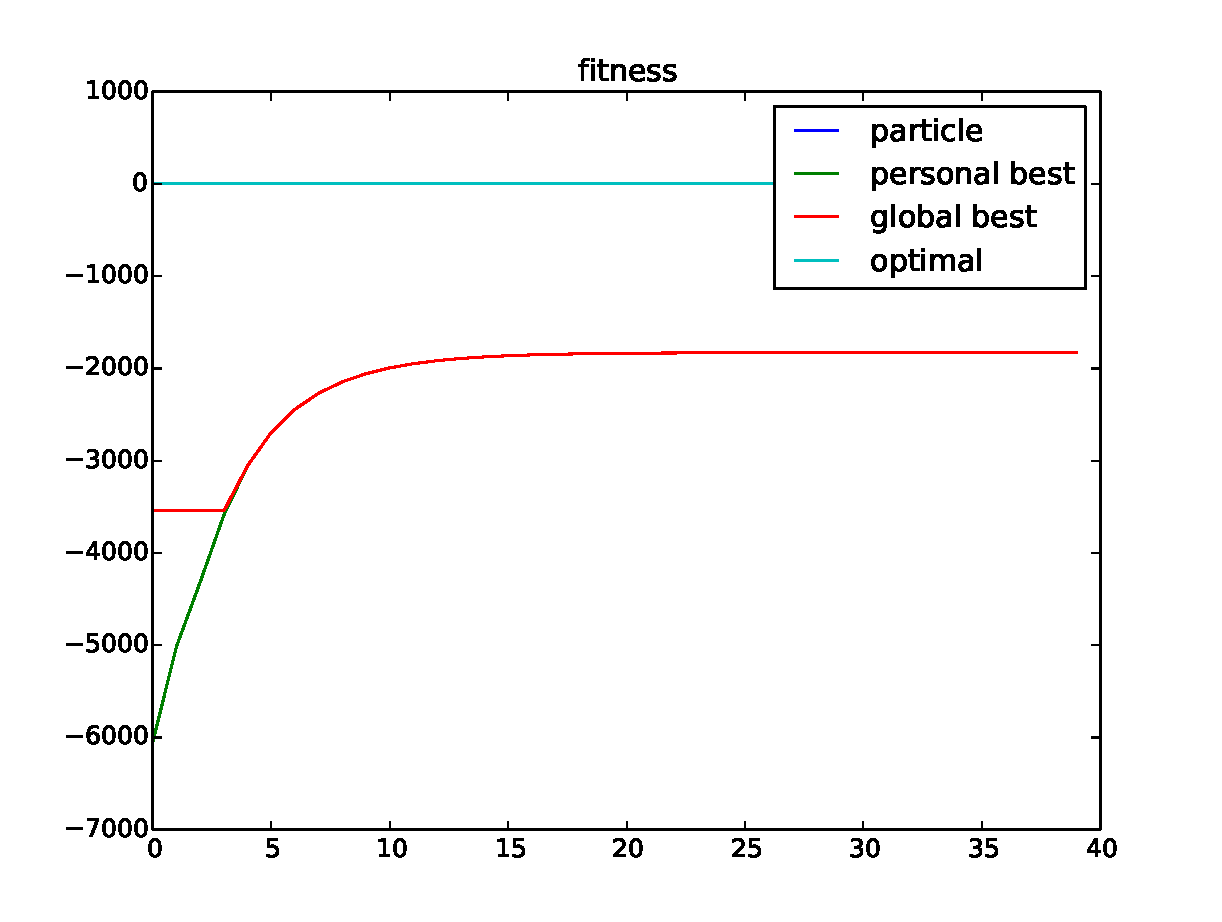
\includegraphics[width=.7\linewidth]{./simfig/case1/fitness1-1} 
\label{fig:case1-1:fitness}
\caption{$ \chi = 0.72984 , \phi^{P} = 2.05 , \phi^{G} = 2.05 $ }
\end{figure}

\begin{figure}[ht]
\centering
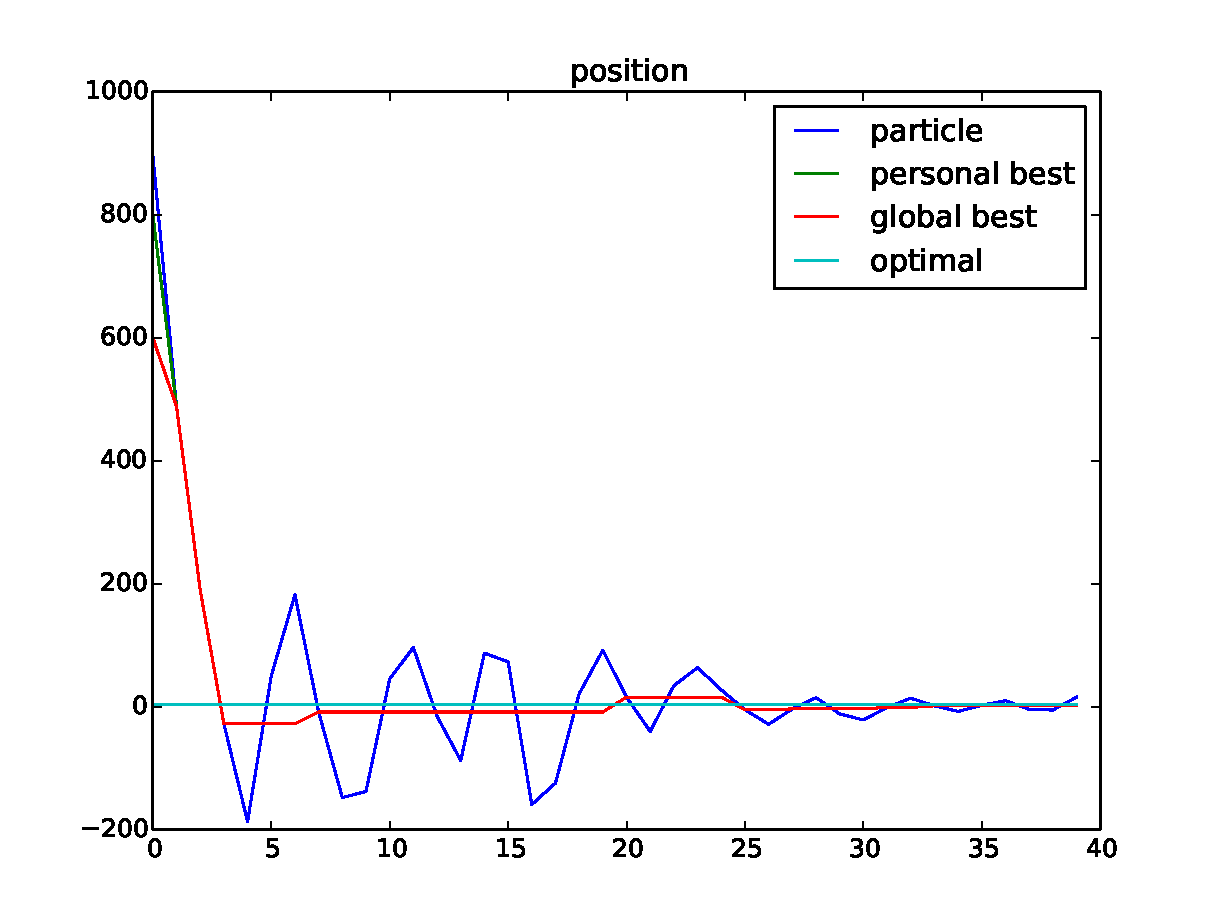
\includegraphics[width=.7\linewidth]{./simfig/case1/position1-2} 
\label{fig:case1-2:position}
\caption{$ \chi = 0.72984 , \phi^{P} = 2.05 , \phi^{G} = 2.05 $ }
\end{figure}
  
\begin{figure}[ht]
\centering
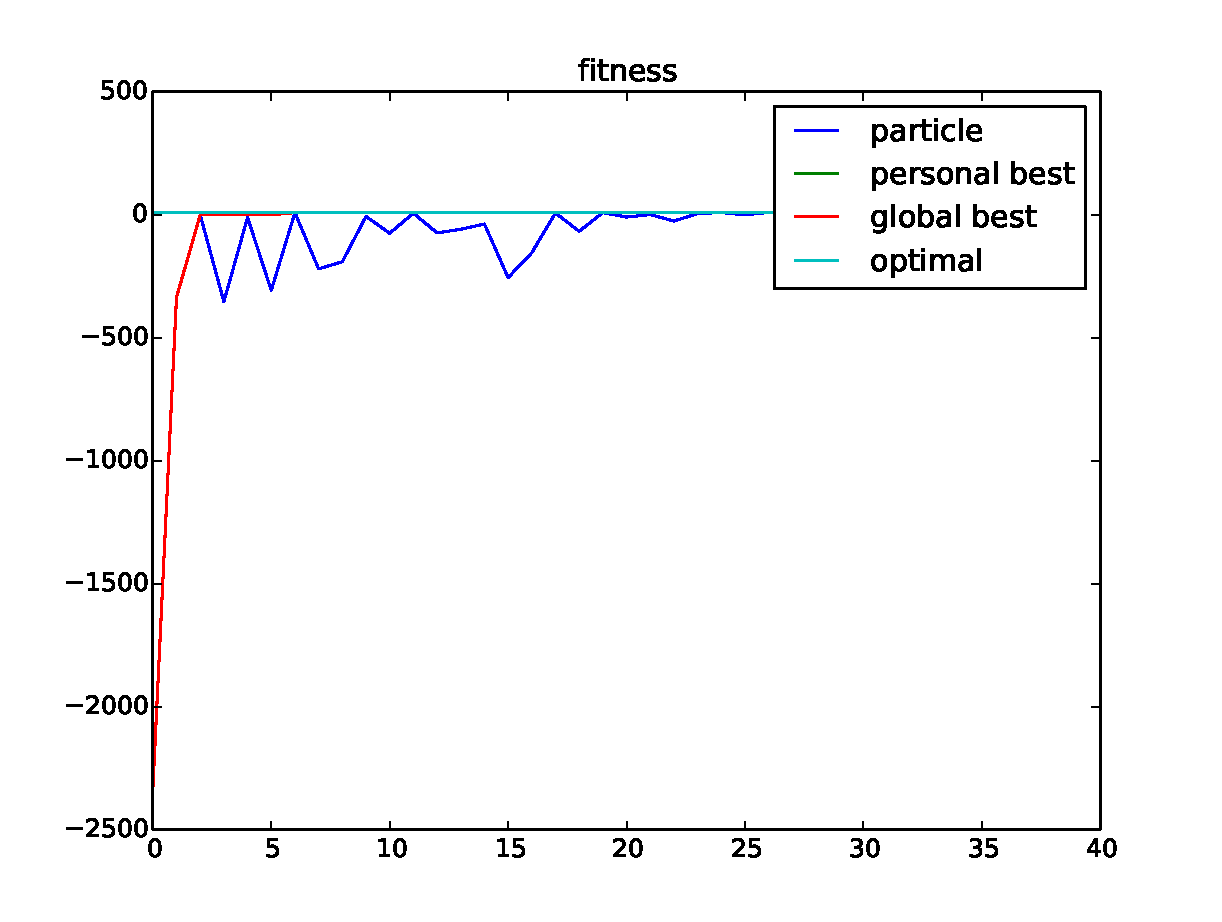
\includegraphics[width=.7\linewidth]{./simfig/case1/fitness1-2} 
\label{fig:case1-2:fitness} 
\caption{$ \chi = 0.72984 , \phi^{P} = 2.05 , \phi^{G} = 2.05 $ }
\end{figure}

\subsubsection{Exploitation}

The convergence property in a unimodal case shows the potential exploitation from the single particle.
As a search heuristic, $ x^{G} $ attracts the particle moving toward itself.


\subsection{Multi-model fitness distribution}

When there is more than one hill in the range that the particle moves, it is not easy to figure out a pattern of the behaviors that the particles share.

[TODO: Give an example that the particle will wander between the personal best and the global best]

As we are interested with the probability that the particle gets into a position that is better than the current global best, we hope the distance from this position to the optimal is closer than that from the global best to the optimal.

In order to measure how likely the particle can moves to a position that $ f(x) > f(x^{G}) $, we can measure the probability of that $ \lVert x(k) - x^{*} \rVert < \lVert x^{G} - x^{*} \rVert $ indirectly.

\begin{mylem}
\label{lem:nonsingleHill:particle:prob}
\begin{equation}
\begin{aligned}
& P( \lVert x(k) - x^{*} \rVert < \lVert x^{G} - x^{*} \rVert ) \\
& > 1 - \frac{ \delta ( \max ( \lVert x^{G} - x^{*} \rVert , \lVert x^{P}(k) - x^{*}  \rVert ) ) }{ \lVert x^{G} - x^{*} \rVert },
\end{aligned}
\end{equation}
in which $ \delta () $ is a boundary function.
\begin{proof}
By Markov's inequality, we have
\begin{equation}
P( \lVert x(k) - x^{*} \rVert \geq \lVert x^{G} - x^{*} \rVert ) \leq \frac{ E( \lVert x(k) - x^{*} \rVert ) }{ \lVert x^{G} - x^{*} \rVert }.
\end{equation} 
By the boundary, we have
\begin{equation}
E( \lVert x(k) - x^{*} \rVert ) \leq \delta ( \max ( \lVert x^{G} - x^{*} \rVert , \lVert x^{P}(k) - x^{*}  \rVert ) ),
\end{equation}
in which $ \delta () $ is the boundary function.
\begin{equation}
\begin{aligned}
& P( \lVert x(k) - x^{*} \rVert < \lVert x^{G} - x^{*} \rVert ) \\
= & 1 - P( \lVert x(k) - x^{*} \rVert \geq \lVert x^{G} - x^{*} \rVert ) \\
> & 1 - \frac{ E( \lVert x(k) - x^{*} \rVert ) }{ \lVert x^{G} - x^{*} \rVert } \\
> & 1 - \frac{ \delta ( \max ( \lVert x^{G} - x^{*} \rVert , \lVert x^{P}(k) - x^{*}  \rVert ) ) }{ \lVert x^{G} - x^{*} \rVert }.
\end{aligned}
\end{equation}
\end{proof}
\end{mylem}

\subsubsection{Simulation on multi-modal cases}

\begin{figure}[ht]
\centering
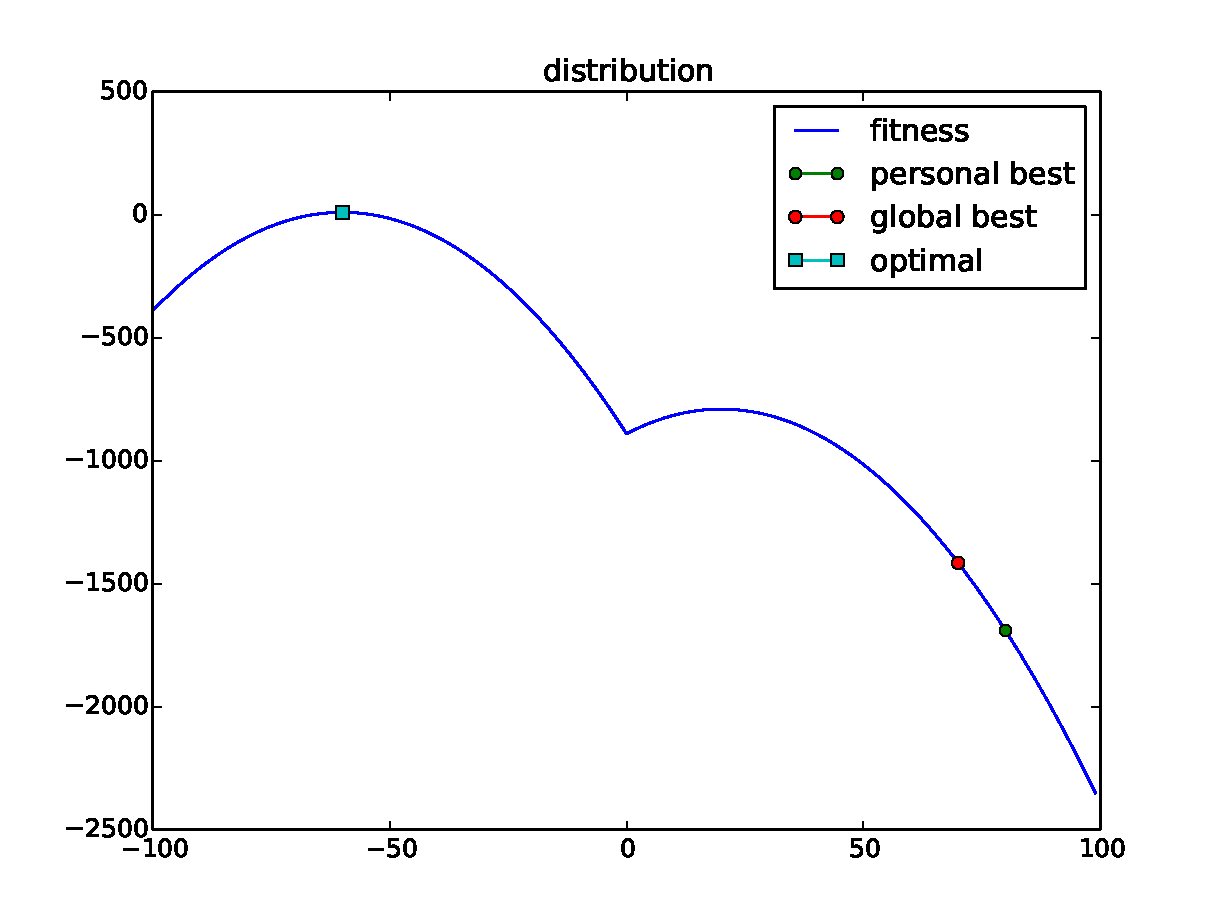
\includegraphics[width=.7\linewidth]{./simfig/case2/distribution2}
\label{fig:case2-1:distribution} 
\end{figure}

\begin{figure}[ht]
\centering
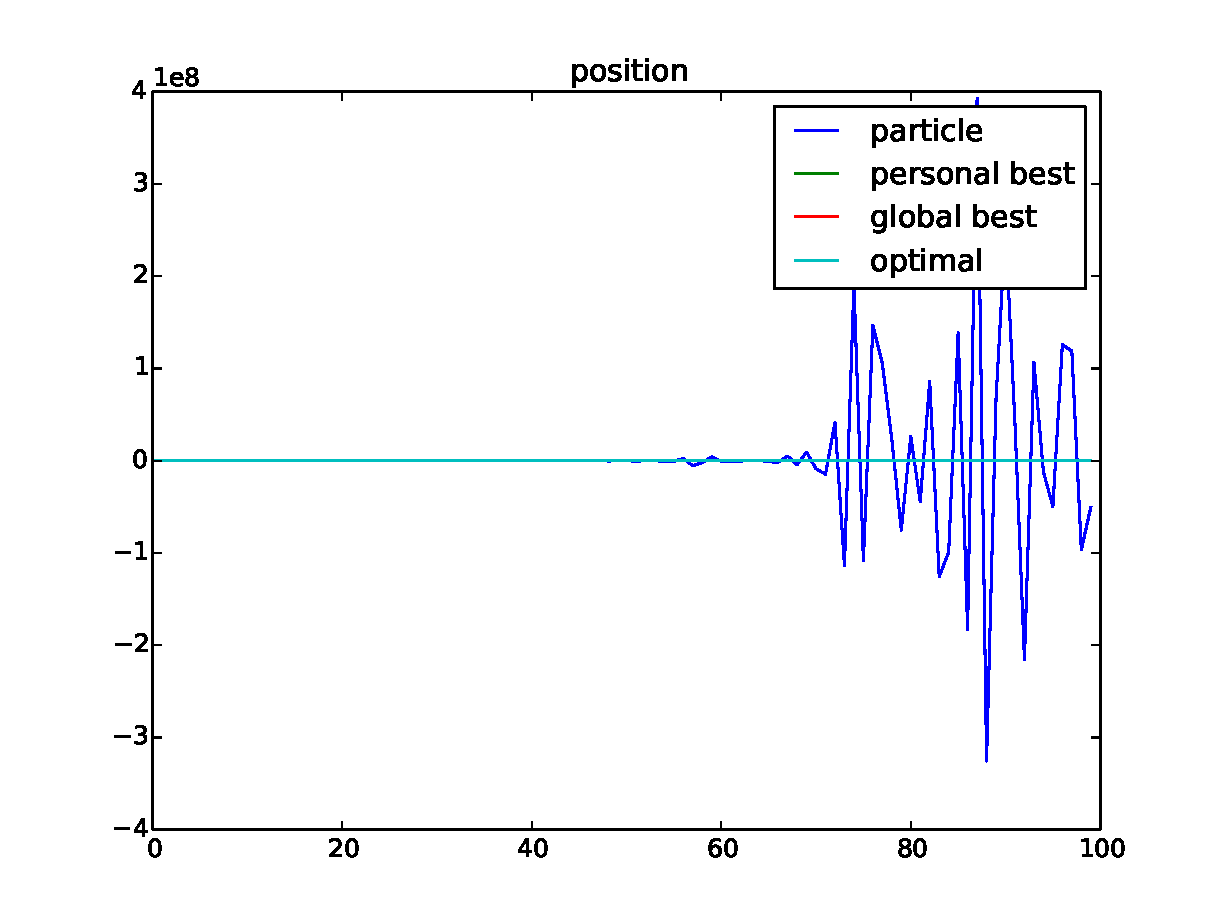
\includegraphics[width=.7\linewidth]{./simfig/case2/position2-1} 
\label{fig:case2-1:position}
\caption{$ \chi = 0.72984 , \phi^{P} = 2.05 , \phi^{G} = 2.05 $ }
\end{figure}

\begin{figure}[ht]
\centering
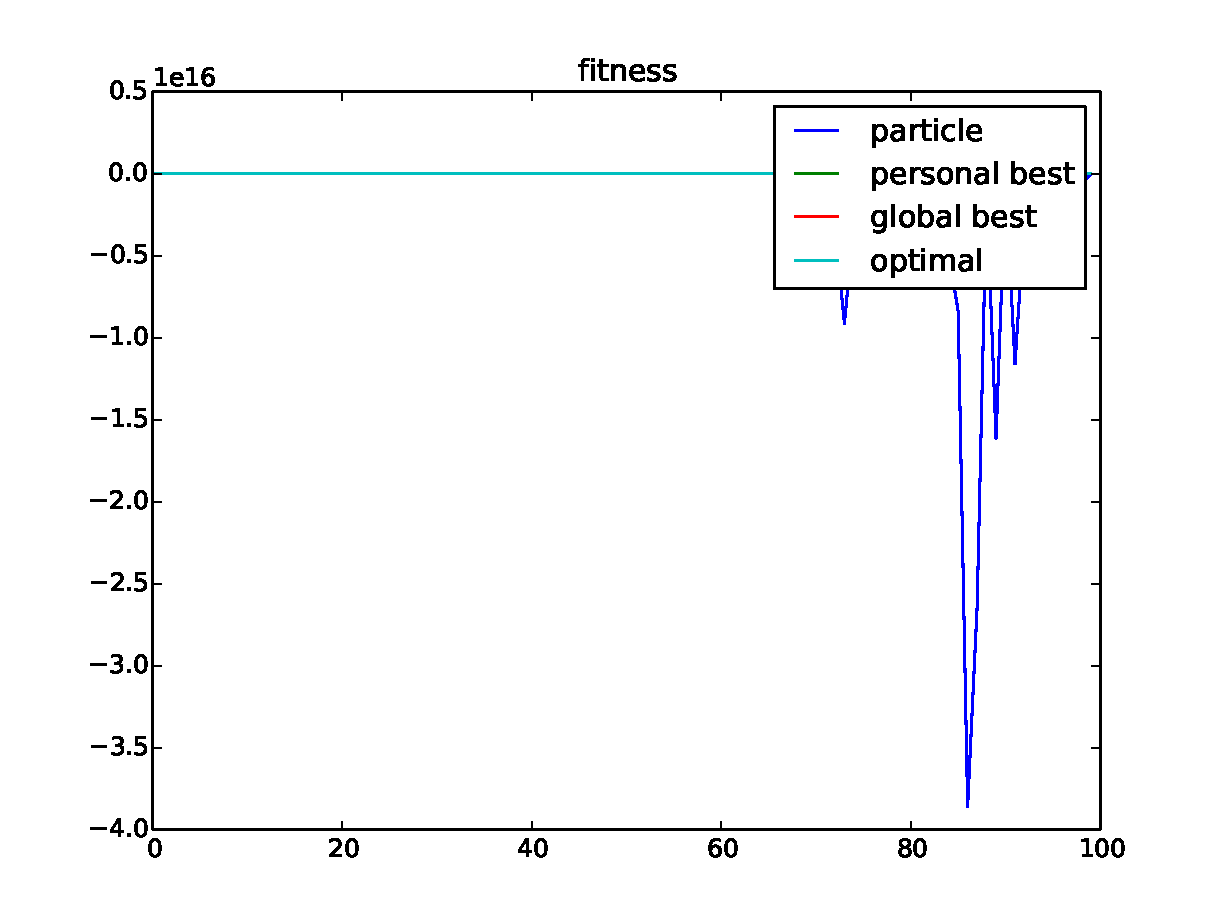
\includegraphics[width=.7\linewidth]{./simfig/case2/fitness2-1} 
\label{fig:case2-1:fitness}
\caption{$ \chi = 0.72984 , \phi^{P} = 2.05 , \phi^{G} = 2.05 $ }
\end{figure}

\begin{figure}[ht]
\centering
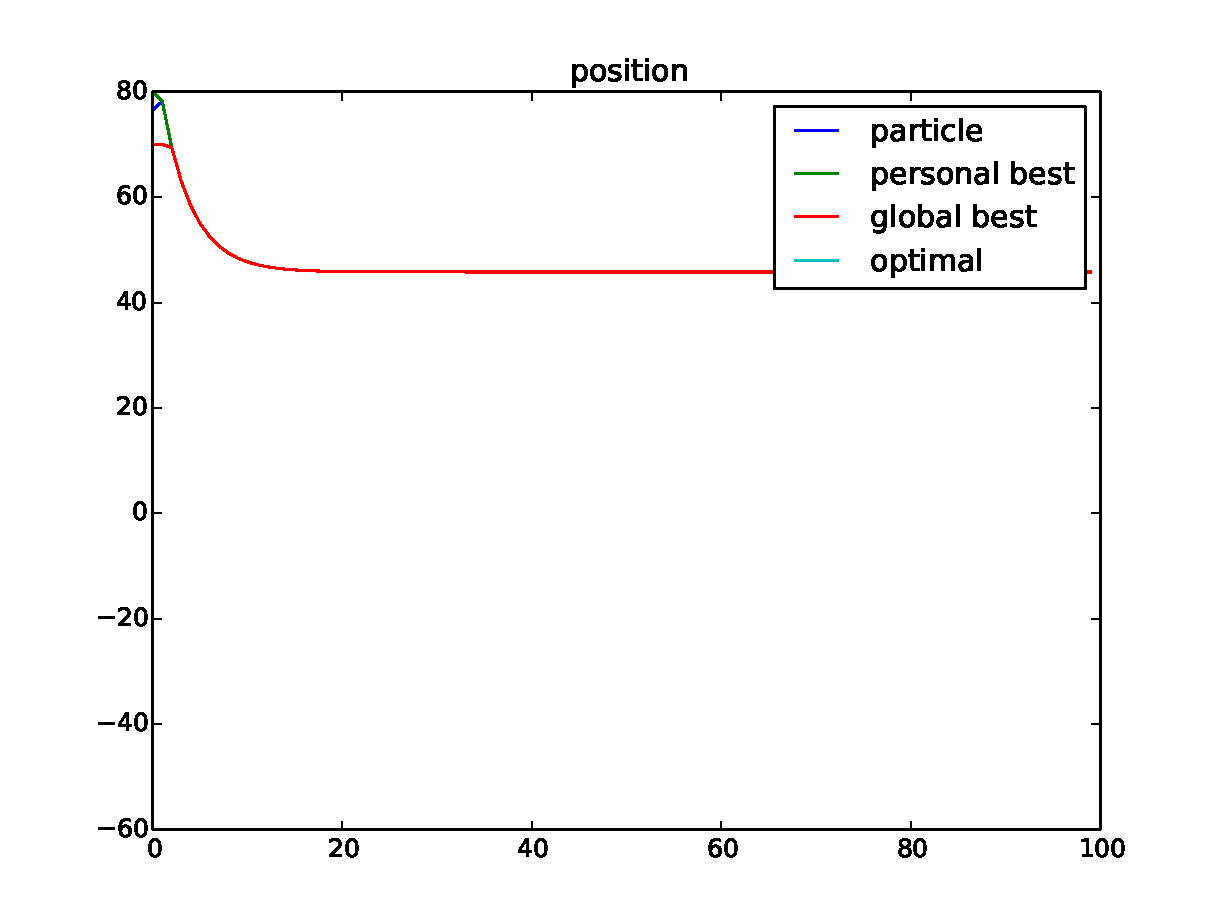
\includegraphics[width=.7\linewidth]{./simfig/case2/position2-2} 
\label{fig:case2-2:position}
\caption{$ \chi = 0.72984 , \phi^{P} = 2.05 , \phi^{G} = 2.05 $ }
\end{figure}
  
\begin{figure}[ht]
\centering
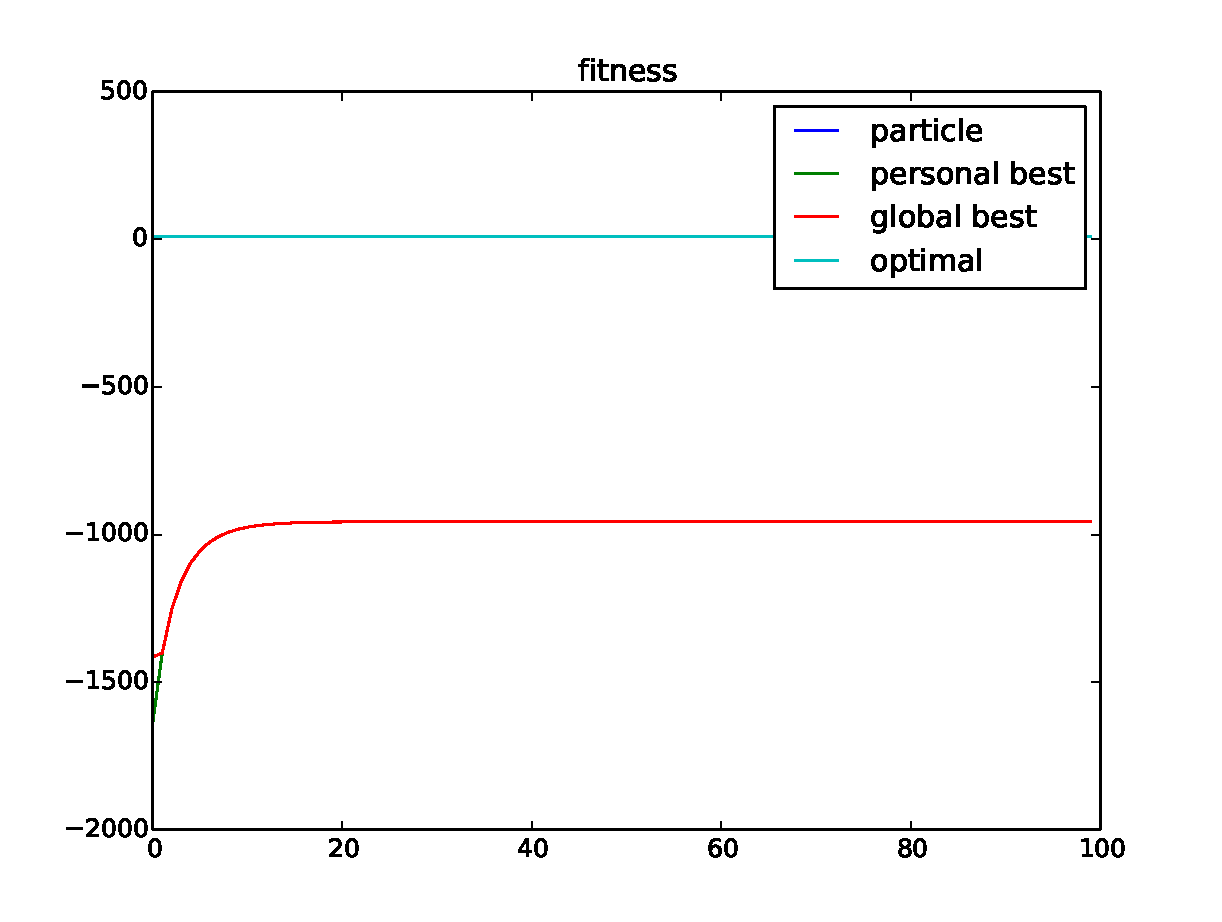
\includegraphics[width=.7\linewidth]{./simfig/case2/fitness2-2} 
\label{fig:case2-2:fitness} 
\caption{$ \chi = 0.72984 , \phi^{P} = 2.05 , \phi^{G} = 2.05 $ }
\end{figure}

\subsubsection{Exploration}


\section{Swarm analysis}
\label{sec:swarm}

%\subsection{Consensus of a swarm}

%\begin{itemize}
%\item Combinations of ISS parts are ISS
%\item Swarm as such a combination
%\item Conditions where update is ISS
%\item trivially at stagnation. But also when on a single hill
%\end{itemize}

%\begin{itemize}
%\item Bound on swarm for the single hill case (perhaps as function of the width of the hill?
%Or width of the hill as a percentage of the feasible region?)
%\item test on 2-d case to show that the bound can prevent a particle from reaching another hill.
%This is one form of the swarm failing to converge the global optimal.
%\item Can we look at parameters for the whole swarm?
%\end{itemize}

\subsection{When the fitness distribution is a single hill}

\begin{mythm}
In one hill case, if there are more than two particles, $ x^{G} \rightarrow x^{*} $.
\begin{proof}
There are two cases, $ x^{G} = x^{*} $ and $ x^{G} \not = x^{*} $
If the global best is $ x^{*} $, the particles will gradually converge to $ x^{*} $ by Lemma \ref{lem:singleHill:particle:nonstop}.
If the global best is not $ x^{*} $, the particles will take turns to find new global best by Theorem \ref{thm:singleHill:particle:better} till $ x^{*} = x^{G} $.
Then it becomes the case $ x^{G} = x^{*} $.
\end{proof}
\end{mythm}

\subsubsection{Simulation}

\subsection{More than single hill case}

\begin{mythm}
The probability that the swarm finds a better global best depends on the probabilities that the particles find better global best, which is
\begin{equation}
P = 1 - \prod_{i=1}^{N} ( 1 - P_{i} ),
\end{equation}
$ P_{i} $ is the probability of particle $ i $ finds a better global best.
\begin{proof}
The search process is a competition among the particles in the swarm.
If the swarm does not find a better global best, it means that none of the particle finds a better global best.
For particle $ i $, the probability that a new global best cannot be found is $ 1 - P_{i} $.
Because the global best is constant, the movements of the particles are independent in the search process.
Thus, the probability that no particle finds a new global best becomes
$ \prod_{i=1}^{N} ( 1 - P_{i} ) $.
Then we can know that the probability that a new global best can be found by the swarm.
\end{proof}
\end{mythm}

\subsubsection{Simulation}

\subsection{Value of a swarm}

%Being on one hill is the unlikely case bound in the multi hill case.
%Might not seem useful but is the essence of what makes a swarm a swarm.
%Bounds the swarm to a region around p-bests where g-best has been unable to pull other particles to its hill.
%For a function with narrow hills, g-bests on a narrow hills is less likely to capture another particle, thus the swarm searches more, for functions with broad hills, p-gest are more likely to be pulled to g-bests hill and search there.
%Thus swarm diversity is the mechanism that allows the swarm to not converge when searching is likely needed but focus and converge when the fitness landscape appear to favor exploitation.
%This does not happen at stagnation and does not happen without multiple members. <need to say this in a more mathematical way>>

%example ?? function for exploration case
%example sphere function for the exploitation case
%try to use bound as a function of hill width metric

%Rastrigin as a counter example? Does it get stuck or just sample for ever? It certainly runs longer.

\subsubsection{Competition}



\subsubsection{Diversity}


\subsection{Diversity injection}

%Work with the Rastrigin function has lead others to experiment with diversity injection to prevent pre-mature convergence (or prevent convergence at all)
%I am not sure, do we want it to converge? ever?
%On what basis would I propose a new algorithm?
%Show that it would converge based on ISS?

\section{Conclusion}
\label{sec:conclusion}

In this paper, we have decomposed the PSO algorithm into a cascade model, which consists of input update and position update components.
We introduce the input-to-state stability analysis to the position update component.
For an input-to-state stable position update component, if the input to this component is bounded, the state is bounded; also if the input to the component converges, the state converges.
The convergence of the PSO is determined by the output of the input update component, which are the personal best and global best.
If they are in stagnation, the particle converges.

The analysis of a cascade structure used here can be applied to a wide range of the PSO variants.
In cases that use the same position update component but different input update components, the convergence and the boundary of the particles are determined by
whether the input update component generates converging or bounded personal best and global best.
For variants that use a different position update component, the ISS properties would need to be verified.


\bibliographystyle{IEEEtran}
\bibliography{reference}

\section*{Appendix}

\subsection{ISS-Lyapunov function}
\label{sec:iss_lyapunov:func}

Using the definitions of a $ K $-function and a $ KL $-function in Section \ref{sec:system}
we can define a ISS-Lyapunov function as follows,
%\begin{itemize}
%\item 
an ISS-Lyapunov function $ V : \mathbb{R}^{n} \rightarrow \mathbb{R}_{\geq 0} $ satisfies:
\begin{enumerate}
\item $ \exists \alpha_{1}, \alpha_{2} \in \mathbb{K} $ such that 
$ \forall \xi \in \mathbb{R}^{n} $ , $ \alpha_{1} ( | \xi | ) \leq V( \xi ) \leq \alpha_{2}  ( | \xi | ) $.
\item $ \exists \alpha_{3} \in \mathbb{K}_{\infty} , \sigma \in \mathbb{K} $ such that $ \forall \xi \in \mathbb{R}^{n}, \forall \mu \in \mathbb{R}^{m} $,$  V( f( \xi, \mu ) ) - V( \xi ) \leq - \alpha_{3} ( | \xi | ) + \sigma ( | \mu | ) $. 
\end{enumerate}

\subsection{Proof of Theorem \ref{thm:iss}}
\label{sec:thm:iss:proof}
		
\begin{proof} 
Let $ P $ be an identity matrix.
As $ | \lambda_{\max} ( A(k) ) | < 1 $, we have
%\begin{equation}
%\nonumber
$
\lVert A^{T}(k) P A(k) \rVert \leq \lVert P \rVert \lVert A(k) \rVert^{2} \leq \lVert P \rVert | \lambda_{\max} ( A(k) ) |^{2} $ $  <  \lVert P \rVert .
$
%\end{equation}
Because $ P $ is an identity matrix it is positive definite, and thus $ A^{T}(k) P A(k) $ is positive definite or positive semi-definite by definition.
So by positive definite ordering we have $ A^{T}(k) P A(k) < P $.
		
Let $ -Q(k) = A^{T}(k) P A(k) - P $. Since $ A^{T}(k) P A(k) < P $ then $ - Q(k) < 0 $ furthermore $ \exists Q' \forall k, Q(k) > Q' > 0 $. 
		
By the Lemma 3.5 in \cite{Jiang2001857}, if we can show that a proposed positive definite Lyapunov function is an ISS-Lyapunov function, then the system is ISS.
		
Define a Lyapunov function
\begin{equation}
\label{eq:lyapunov_v}
V( X(k) ) = X^{T} (k) P X(k).
\end{equation}
We can have
$
\lambda_{min}(P) | X(k) |^{2} \leq V( X(k) )\leq \lambda_{max}(P) | X(k) |^{2}
$ and $ \lambda_{min}(P) = \lambda_{max}(P) $.
		
Let $ \alpha_{1} ( \xi )= \lambda_{min} \xi^{2} $
and 
$ \alpha_{2} ( \xi )= \lambda_{max} \xi^{2} $,
we have $ V(x) $ satisfying condition 1 of the ISS-Lyapunov function definition.
		
By applying equation \eqref{eq:pso_up_linalg_simp} to $ V( X(k+1) ) - V( X(k) ) $, we have
\begin{equation}
\label{eq:lyapunov_delta2}
\begin{aligned}
& V( X(k+1) ) - V( X(k) ) \\
%	= & - X^{T}(k) [ A^{T}(k) P A(k) - P ] X(k) + 2 X^{T}(k)  A^{T}(k) P B(k) U(k) \\
%	& + U^{T}(k) B^{T}(k) P B(k) U(k) \\
%	\leq & - X^{T}(k) Q' X(k) + 2 X^{T}(k)  A^{T}(k) P B(k) U(k) \\
%	& + U^{T}(k) B^{T}(k) P B(k) U(k) \\
%	\leq & - \lambda_{min}(Q') | X(k) |^{2} + 2  \lVert A^{T}(k) P B(k) \rVert  U(k) | | X(k) | \\
%	& + \lVert B^{T}(k) P B(k) \rVert | U(k) |^{2}.
= & [ X^{T}(k)  A^{T}(k) + U^{T}(k) B^{T}(k) ] P [ A(k) X(k) + B(k) U(k) ] \\ & - X^{T}(k) P X(k) \\
= & X^{T}(k)  A^{T}(k) P A(k) X(k) +  X^{T}(k)  A^{T}(k) P B(k) U(k) \\
& + U^{T}(k) B^{T}(k) P A(k) X(k) + U^{T}(k) B^{T}(k) P B(k) U(k) \\ & - X^{T}(k) P X(k) \\
\end{aligned}
\end{equation}
As $ P $ is identity matrix, it is symmetric, thus
\begin{equation}
[ X^{T}(k)  A^{T}(k) P B(k) U(k) ]^{T} =  U^{T}(k) B^{T}(k) P A(k) X(k).
\end{equation}
$ V( X(k+1) ) , V( X(k) ) \in \mathbb{R} $, 
we have $ X^{T}(k)  A^{T}(k) P B(k) U(k) $ and $  U^{T}(k) B^{T}(k) P A(k) X(k) $ are both real value (like $ 1 \times 1 $ matrix).
Thus, 
\begin{equation}
 X^{T}(k)  A^{T}(k) P B(k) U(k) =   U^{T}(k) B^{T}(k) P A(k) X(k) .
\end{equation}
We then have
\begin{equation}
\label{eq:lyapunov_delta3}
\begin{aligned}
& V( X(k+1) ) - V( X(k) ) \\
= & - X^{T}(k) [ A^{T}(k) P A(k) - P ] X(k) \\
& + U^{T}(k) B^{T}(k) P B(k) U(k)  \\
& + 2 X^{T}(k)  A^{T}(k) P B(k) U(k) \\
\leq & - X^{T}(k) Q' X(k)  + U^{T}(k) B^{T}(k) P B(k) U(k) \\
& + 2 X^{T}(k)  A^{T}(k) P B(k) U(k) \\
\end{aligned}
\end{equation}

By applying matrix norm, we have
\begin{equation}
\begin{aligned}
& V( X(k+1) ) - V( X(k) ) \\
\leq & - \lambda_{min}(Q') | X(k) |^{2}  + | B^{T}(k) P B(k) | | U(k) |^{2} \\
& + 2  | A^{T}(k) P B(k) | | U(k) | | X(k) | \\
= & - \frac{1}{2} \lambda_{min}(Q') | X(k) |^{2} + | B^{T}(k) P B(k) | | U(k) |^{2} \\
& - \frac{1}{2} \lambda_{min}(Q') | X(k) |^{2} + 2  | A^{T}(k) P B(k) | | U(k) | | X(k) |  \\
= & - \frac{1}{2} \lambda_{min}(Q') | X(k) |^{2} \\
& + \left( \frac{2 | A^{T}(k) P B(k) |^{2}}{ ( \lambda_{min}(Q') )^{2} } + | B^{T}(k) P B(k) |  \right) | U(k) |^{2} \\
& - \frac{1}{2} \lambda_{min}(Q') [ | X(k) |^{2} - \frac{4 | A^{T}(k) P B(k) | }{ \lambda_{min}(Q') }  | X(k) | | U(k) | \\
& + \frac{4 | A^{T}(k) P B(k) |^{2}}{ ( \lambda_{min}(Q') )^{2} } | U(k) |^{2} ] \\
\end{aligned}
\end{equation}
		
By completing the square, we have
\begin{equation}
\label{eq:lyapunov_delta4}
\begin{aligned}
& V( X(k+1) ) - V( X(k) ) \\
= & - \frac{1}{2} \lambda_{min}(Q') | X(k) |^{2} \\
& + \left( \frac{2 | A^{T}(k) P B(k) |^{2}}{ ( \lambda_{min}(Q') )^{2} } + | B^{T}(k) P B(k) | \right) | U(k) |^{2} \\
& - \frac{1}{2} \lambda_{min}(Q') \left( | X(k) | - \frac{2 | A^{T}(k) P B(k) | }{ \lambda_{min}(Q') } | U(k) | \right)^{2} \\
	\leq & - \frac{1}{2} \lambda_{min}(Q') | X(k) |^{2} \\
 &	+ \left( \frac{2 \lVert A^{T}(k) P B(k) \rVert^{2}}{ ( \lambda_{min}(Q') )^{2} } 
	 + \lVert B^{T}(k) P B(k) \rVert \right) | U(k) |^{2}. 
\end{aligned}
\end{equation}
		
Because $ u^{P}(k) \in [0, 1] $, there exist an $ A' $ and $ B' $ such that $ \lVert A(k) \rVert \leq \lVert A' \rVert $ and $ \lVert B(k) \rVert \leq \lVert B' \rVert $.
We have $ \lVert A^{T}(k) P B(k) \rVert $ $  \leq \lVert A' \rVert \lVert P \rVert \lVert B' \rVert $ and $ \lVert B^{T}(k) P B(k) \rVert \leq \lVert P \rVert \lVert B' \rVert^{2} $.
		
Since the identity matrix $ P $ has $ || P || = 1 $:
\begin{equation}
\label{eq:lyapunov_delta5}
\begin{aligned}
& V( X(k+1) ) - V( X(k) ) \\
	\leq & - \frac{1}{2} \lambda_{min}(Q') | X(k) |^{2} + \left( \frac{2 \lVert A' \rVert^{2} \lVert B' \rVert^{2}}{ ( \lambda_{min}(Q') )^{2} } + \lVert B' \rVert^{2} \right) | U(k) |^{2}.
\end{aligned}
\end{equation}
		
Let
\begin{equation}
\nonumber
\alpha_{3} ( \xi )= \frac{1}{2} \lambda_{min}(Q') \xi^{2} ,
\end{equation}
and
\begin{equation}
\nonumber
\sigma ( \xi ) = \left( \frac{2 \lVert A' \rVert^{2} \lVert B' \rVert^{2}}{ ( \lambda_{min}(Q') )^{2} } +  \lVert B' \rVert^{2} \right) \xi^{2} .
\end{equation} 
Thus we have $  V( X(k+1) ) - V( X(k) ) $ satisfying condition 2 of the ISS-Lyapunov function definition and
so \eqref{eq:lyapunov_v} is an ISS-Lyapunov function.
Using Jiang's Lemma 3.5\cite{Jiang2001857}, the position-update component of PSO (equation \eqref{eq:pso_up_linalg_simp}) is input-to-state stable.
\end{proof}

\subsection{Proof of Corollary \ref{coro:param_unit_disc}}
\label{sec:coro:param_unit_disc:proof}

\begin{proof}
Let $ a = (1 + \chi) - \chi \phi $. 
The eigenvalues of $ A(k) $ are
\begin{equation}
\nonumber
 \lambda = \frac{ a \pm \sqrt{ a^{2} - 4 \chi } }{2} .
\end{equation}
There can be two cases.		
\begin{enumerate}
\item If $ a^{2} \geq 4 \chi $, the eigenvalues are complex number.
We have $ a \geq 2 \sqrt{\chi} $ or $ a \leq - 2 \sqrt{\chi} $.
			
If $ a \geq 2 \sqrt{\chi} $, then $ | \lambda_{\max} | < 1 $ derives 
\begin{equation}
\nonumber
0 < \frac{a-\sqrt{a^{2}-4\chi}}{2} \leq \frac{a+\sqrt{a^{2}-4\chi}}{2} < 1 .
\end{equation}
It means that $ 2 \sqrt{ \chi } \leq a < 1 + \chi $.
			
If $ a \leq 2 \sqrt{\chi} $, then $ | \lambda_{\max} | < 1 $ derives
\begin{equation}
\nonumber
-1 < \frac{a-\sqrt{a^{2}-4\chi}}{2} \leq \frac{a+\sqrt{a^{2}-4\chi}}{2} < 0 .
\end{equation}
It means that $ - (\chi+1) < a \leq - 2 \sqrt{\chi} $.
			
\item If $ a^{2} < 4 \chi $, the eigenvalues are real number.
We have $ - 2 \sqrt{\chi} < a < 2 \sqrt{\chi} $.
			
$ | \lambda_{\max} | < 1 $ derives
\begin{equation}
\nonumber
\frac{ a^{2} }{4} + \frac{ a^{2} - 4\chi }{4} < 1 .
\end{equation}
It means that $ - 2 \sqrt{ 2(1+\chi) } < a < 2 \sqrt{ 2(1+\chi) } $.
Because $ \sqrt{ 2(1+\chi) } > 2 \sqrt{ \chi } $, we have $ - 2 \sqrt{\chi} < a < 2 \sqrt{\chi} $.
\end{enumerate}
Combining these two cases, we have  $ - (1 + \chi) < a < 1 + \chi $.
It equals to $ \phi \in \left( 0 , \frac{2(1+\chi)}{\chi} \right) $.
\end{proof}	

\subsection{Proof of the Theorem \ref{thm:state_bound}}	
\label{sec:thm:state_bound:proof}

\begin{proof}
As we have the update equation as
$ X(k+1) = A(k) X(k) + B(k) U(k) $, we can derive 
\begin{equation}
X(k+1) = ( \prod_{k}^{i=0} A(i) ) X(0) + \sum_{i=0}^{k} [ ( \prod_{j=0}^{i-1} A(j) ) B(i) U(i)  ] 
\end{equation}
by recursively applying it.

By the property of matrix norm, we have
\begin{equation}
| X(k+1) | \leq ( \prod_{i=0}^{k} \lVert A(i) \rVert ) | X(0) | + \sum_{i=0}^{k} [ ( \prod_{j=0}^{i-1} \lVert A(j) \rVert ) \lVert B(i) \rVert | U(i) |  ].
\end{equation}

$ \forall i \in [0, k] $, let $ \lVert A(i) \rVert \leq \lVert A \rVert $, $  \lVert B(i) \rVert \leq \lVert B \rVert $ and $ | U(k) | = [ x^{G}(k) - x^{R}, x^{P}(k) - x^{R} ]^{T} $, we have
\begin{equation}
\label{eq:bound:final}
\begin{aligned}
& |  x(k+1) - x^{R} | \leq | X(k+1) | \\
& \leq ( \lVert A \rVert )^{k+1} | X(0) | + \sum_{i=0}^{k} [ ( \lVert A \rVert )^{i} \lVert B \rVert | U(i) |  ] \\
& = ( \lVert A \rVert )^{k+1} | X(0) | + \frac{1 - ( \lVert A \rVert )^{k+1} }{1 - \lVert A \rVert }  \lVert B \rVert | U(i) |
\end{aligned}
\end{equation}

%The boundary will be a function of $ bound ( \lVert A \rVert, \lVert B \rVert, | X(0) |, | U |, k ) $.
%Thus the minimum boundary is $ \min_{k} bound ( \lVert A \rVert, \lVert B \rVert, | X(0) |, | U |, k ) $.
%When we have $ \lVert A \rVert < 1 $, 
%$ ( \lVert A \rVert )^{k+1} \rightarrow 0 $ and
%$ \frac{1 - (\lVert A \rVert )^{k+1} }{1 - \lVert A \rVert} \rightarrow \frac{1}{1 - \lVert A \rVert } $
%as $ k \rightarrow \infty $.

$ ( \lVert A \rVert )^{k+1} $ shows the decay term and $ \frac{1 - ( \lVert A \rVert )^{k+1} }{1 - \lVert A \rVert }  \lVert B \rVert $ makes the boundary function $ \gamma () $.
\end{proof}


\subsection{Mean model of the position update component}
\label{app:mean_pso}

By applying mean to \eqref{eq:pso_up_linalg_simp}, we can have the mean of the position update component as
\begin{equation}
\label{eq:pso_up_linalg_simp:mean}
E( X(k+1) ) = A(k) E( X(k) ) + B(k) E( U(k) )
\end{equation}
with
$ A(k) = \begin{bmatrix}
\chi & - \chi \phi^{G}/2 - \chi \phi^{P}/2
\\ 
\chi & 1 - \chi \phi^{G}/2 - \chi \phi^{P}/2
\end{bmatrix} $
and
$ B(k) = \begin{bmatrix}
\chi \phi^{G}/2 & \chi \phi^{P}/2
\\ 
\chi \phi^{G}/2 & \chi \phi^{P}/2
\end{bmatrix} $.

$ E( X(k) ) = [ E( v(k) ), E( x(k) - x^{R} ) ]^{T} $ and $ E( U(k) ) = [ E( x^{G}(k) - x^{R} ) , E( x^{P}(k) - x^{R} ) ]^{T} $.

By taking $ x^{R} = x^{*} $, we can have \eqref{eq:mean:opt_bound}.

\subsection{Proof of Corollary \ref{coro:param_unit_disc:mean}}
\label{sec:coro:param_unit_disc:proof:mean}

\begin{proof}
The proof is similar with that in Subsection \ref{sec:coro:param_unit_disc:proof}.
In this case, $ a = (1 + \chi) - \frac{ \phi }{2} \chi $.
Similarly, we can have two cases and derive
$ - (1 + \chi) < a < 1 + \chi $.
It equals to 
$
\phi \in \left( 0 , \frac{4(1+\chi)}{\chi} \right) .
$
\end{proof}

\end{document}

